\documentclass[11pt,a4paper]{article}
\usepackage[T1]{fontenc}
\usepackage[utf8]{inputenc}
\usepackage{lmodern}
\usepackage[margin=22mm,headheight=16pt]{geometry}
\usepackage{amsmath,amssymb,graphicx,array,longtable,booktabs}
\usepackage{microtype,xcolor,hyperref,xurl,fancyhdr}
\definecolor{Navy}{HTML}{17324D}
\definecolor{Teal}{HTML}{087F8C}
\definecolor{Gold}{HTML}{B88128}
\hypersetup{colorlinks=true,linkcolor=Navy,urlcolor=Teal,bookmarksnumbered=true,hypertexnames=false}
\setlength{\parindent}{0pt}
\setlength{\parskip}{6pt}
\setlength{\emergencystretch}{4em}
\setcounter{tocdepth}{1}
\pagestyle{fancy}\fancyhf{}
\fancyfoot[R]{\small\thepage}
\fancyfoot[L]{\small\sffamily Sharif University of Technology}
\renewcommand{\headrulewidth}{0.3pt}
\makeatletter
\renewcommand\section{\@startsection{section}{1}{\z@}{-3.2ex plus -1ex minus -.2ex}{1.6ex plus .2ex}{\normalfont\Large\sffamily\bfseries\color{Navy}}}
\renewcommand\subsection{\@startsection{subsection}{2}{\z@}{-2.5ex plus -1ex minus -.2ex}{1.2ex plus .2ex}{\normalfont\large\sffamily\bfseries\color{Teal}}}
\makeatother
\fancyhead[L]{\small\sffamily\color{Navy}Reza Sanaee Nezhad}\fancyhead[R]{\small\sffamily\color{Teal}Technical Report}\begin{document}
\begin{titlepage}\centering\vspace*{7mm}

\includegraphics[width=31mm]{assets/sharif_emblem_en.png}\par\vspace{5mm}
{\Large\sffamily\bfseries\color{Navy}SHARIF UNIVERSITY OF TECHNOLOGY\par}
\vspace{2mm}{\sffamily Department of Electrical Engineering\par}
\vspace{17mm}{\color{Teal}\rule{\linewidth}{1.4pt}}\par\vspace{6mm}
{\large\sffamily\color{Teal}TECHNICAL REPORT\par}
\vspace{8mm}{\huge\sffamily\bfseries\color{Navy}Single-Node Hadoop and Spark Deployment with Distributed Word Count\par}
\vspace{9mm}{\color{Gold}\rule{45mm}{1pt}}\par\vfill
\begin{minipage}{.88\linewidth}{\sffamily\color{Teal}AUTHOR}\par{\Large\sffamily Reza Sanaee Nezhad}\par Student ID: 401101502\par\vspace{7mm}
{\sffamily\color{Teal}INSTRUCTOR / INSTRUCTORS}\par
Dr Iman Gholampour\par\vspace{7mm}
{\sffamily\color{Teal}ACADEMIC CONTEXT}\par
Big Data Processing\par\end{minipage}\vfill
\end{titlepage}
\tableofcontents\clearpage
\section{Processing model and Spark abstractions}

Batch processing operates on a bounded dataset and suits historical analysis, ETL, and offline training. Streaming operates on an unbounded input and continuously produces updated results, often through micro-batches. Latency depends on ingestion, trigger interval, computation, and scheduling;\allowbreak{} calling a pipeline streaming does not establish a millisecond deadline. An RDD is an immutable partitioned distributed collection with lineage for recovery. Transformations construct a lazy computation graph;\allowbreak{} actions trigger execution. RDDs remain useful for custom low-level transformations and assignment constraints. They do not require the entire dataset to reside in RAM, and a lost partition can often be recomputed from its lineage. DataFrames expose named columns and a schema, allowing query optimization. Datasets add a typed interface in languages such as Scala and Java;\allowbreak{} Python does not have the same typed Dataset API. Type safety is not a guarantee against every runtime error, and optimization benefits depend on the operation used. The driver constructs the application, plans work, and coordinates jobs, stages, and tasks. The cluster manager allocates resources. Executors run tasks and may cache partitions. A shuffle redistributes data by key and can incur network transfer, serialization, disk I/\allowbreak{}O, and skew. reduceByKey can combine values locally before shuffle, whereas groupByKey usually transfers the raw grouped values.

\begin{figure}[!htbp]\centering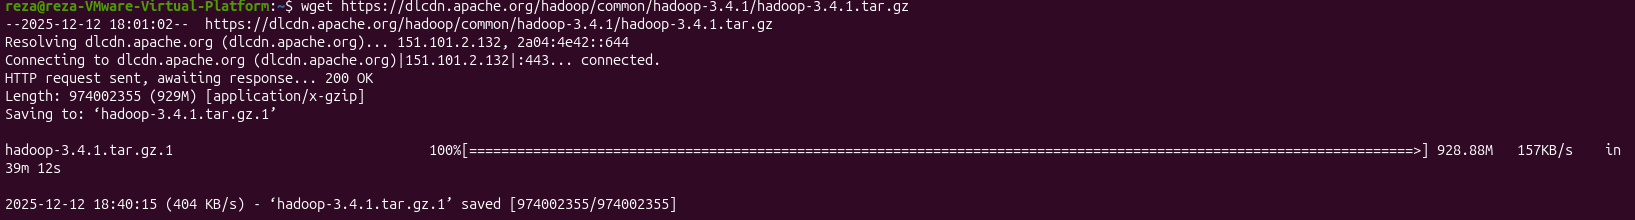
\includegraphics[width=\linewidth,height=.72\textheight,keepaspectratio]{assets/041_p010_02.png}\caption{Diagram or recorded result: Processing model and Spark abstractions.}\label{fig:041_p010_020}\end{figure}
\begin{figure}[!htbp]\centering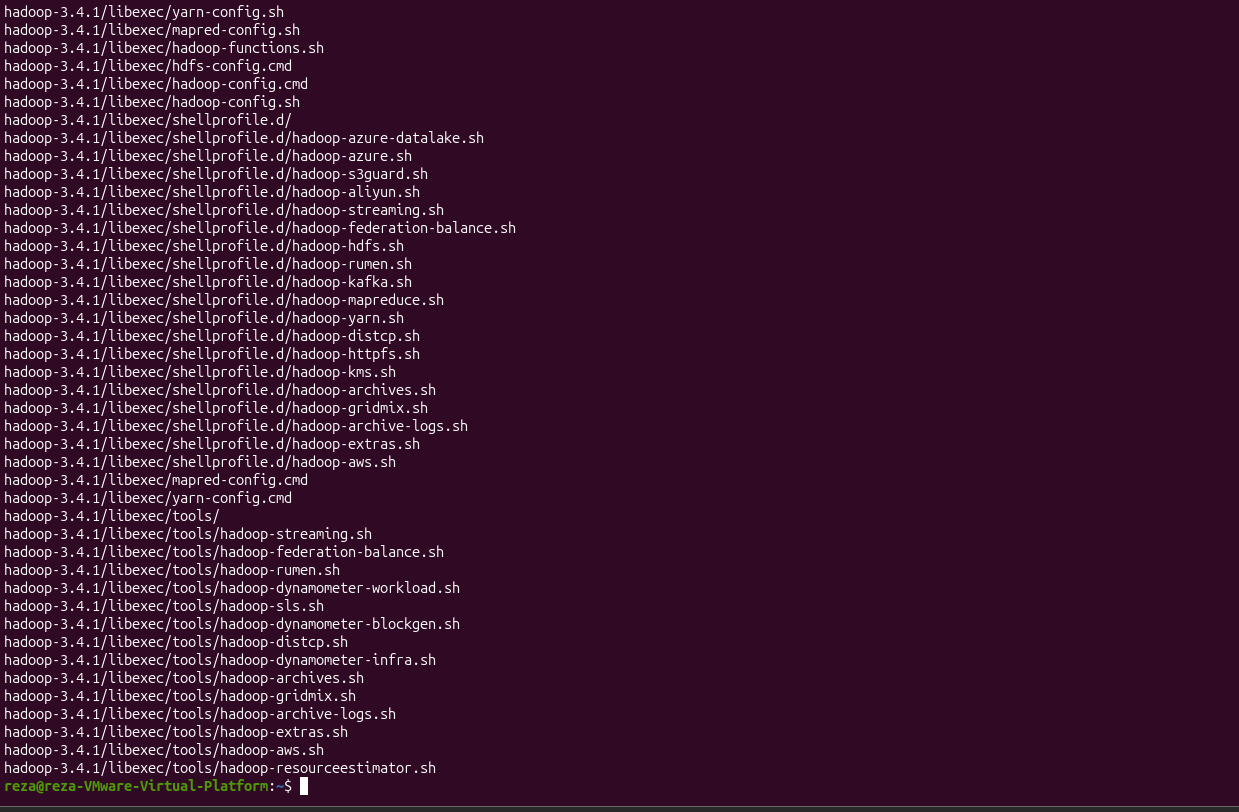
\includegraphics[width=\linewidth,height=.72\textheight,keepaspectratio]{assets/041_p010_03.png}\caption{Diagram or recorded result: Processing model and Spark abstractions.}\label{fig:041_p010_030}\end{figure}
\begin{figure}[!htbp]\centering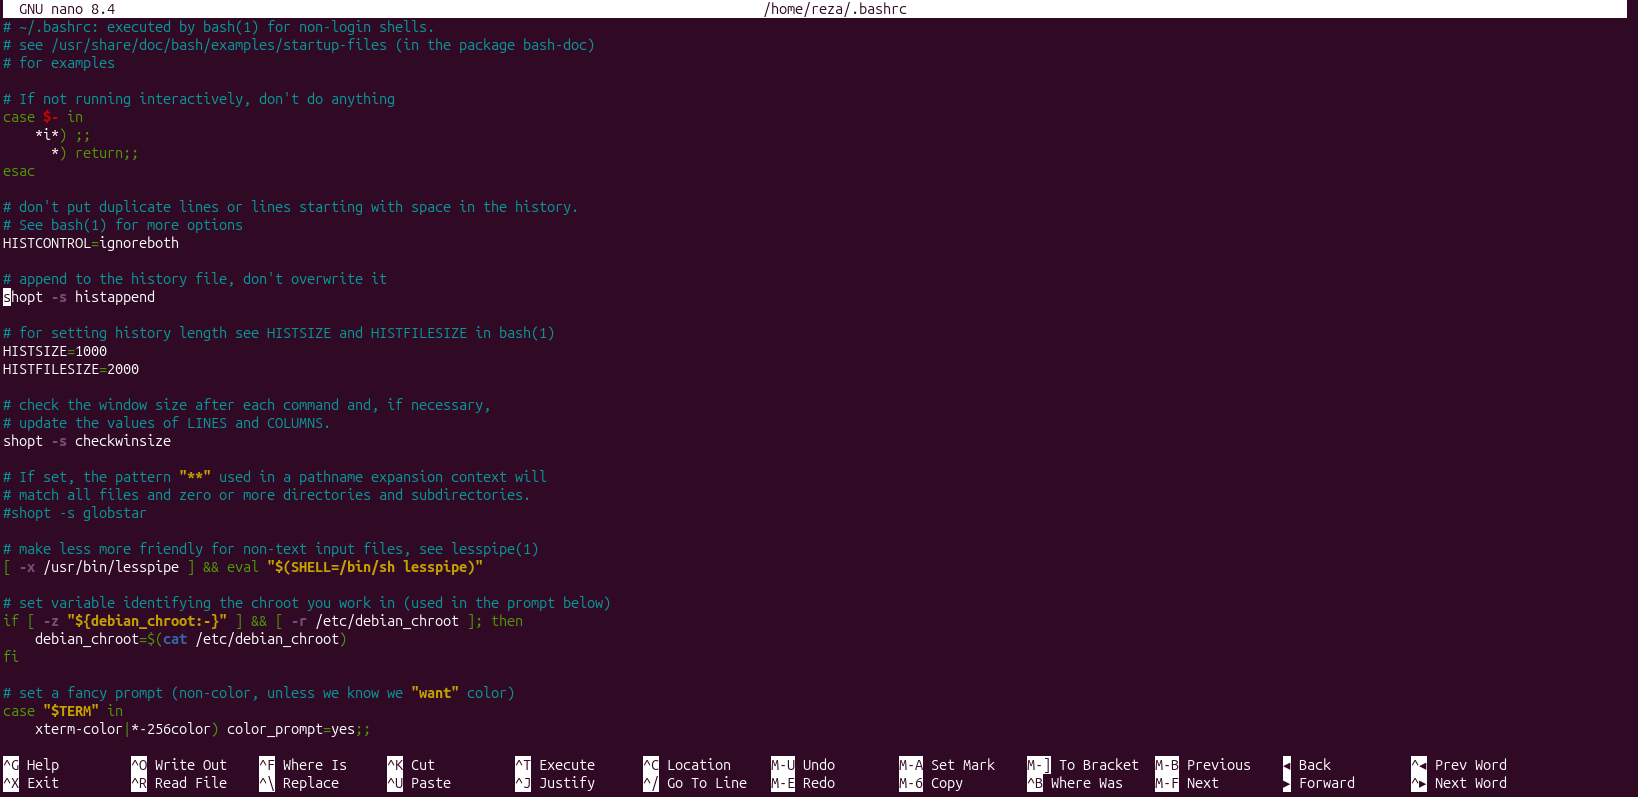
\includegraphics[width=\linewidth,height=.72\textheight,keepaspectratio]{assets/041_p011_01.png}\caption{Diagram or recorded result: Processing model and Spark abstractions.}\label{fig:041_p011_010}\end{figure}
\begin{figure}[!htbp]\centering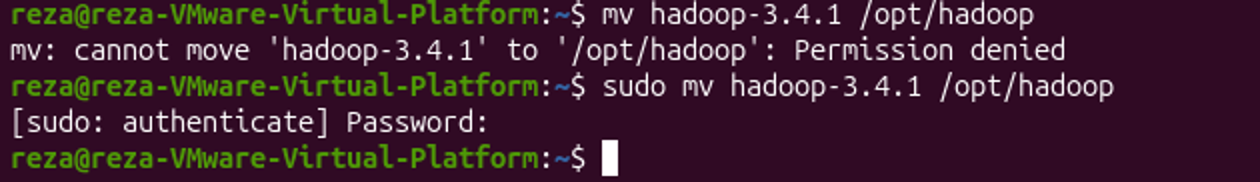
\includegraphics[width=\linewidth,height=.72\textheight,keepaspectratio]{assets/041_p011_02.png}\caption{Implementation and output: Processing model and Spark abstractions.}\label{fig:041_p011_020}\end{figure}
\begin{figure}[!htbp]\centering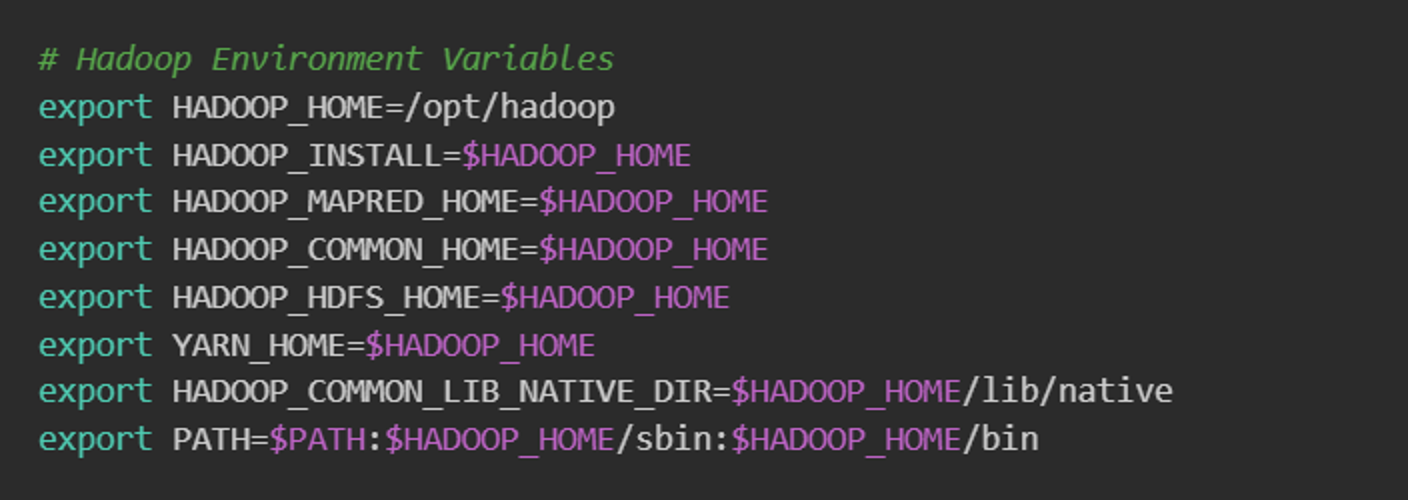
\includegraphics[width=\linewidth,height=.72\textheight,keepaspectratio]{assets/041_p012_01.png}\caption{Diagram or recorded result: Processing model and Spark abstractions.}\label{fig:041_p012_010}\end{figure}
\begin{figure}[!htbp]\centering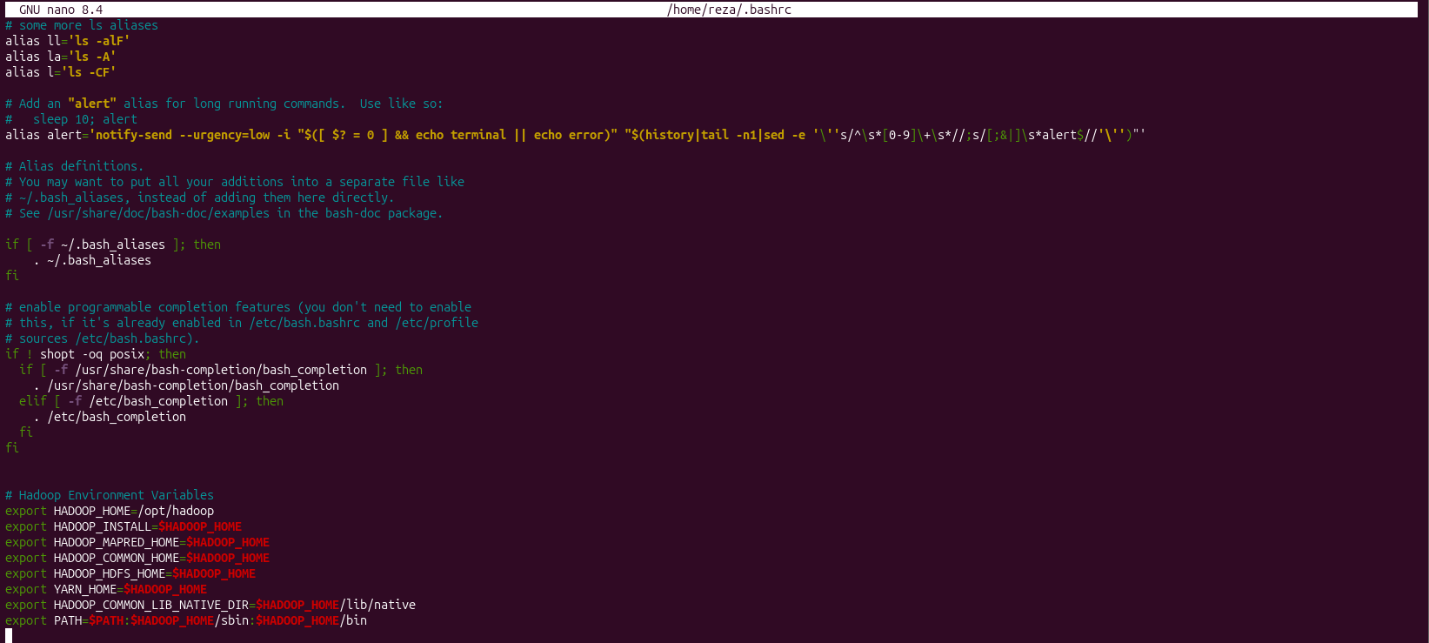
\includegraphics[width=\linewidth,height=.72\textheight,keepaspectratio]{assets/041_p012_02.png}\caption{Diagram or recorded result: Processing model and Spark abstractions.}\label{fig:041_p012_020}\end{figure}
\begin{figure}[!htbp]\centering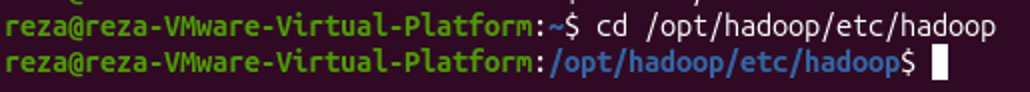
\includegraphics[width=\linewidth,height=.72\textheight,keepaspectratio]{assets/041_p012_03.png}\caption{Diagram or recorded result: Processing model and Spark abstractions.}\label{fig:041_p012_030}\end{figure}
\begin{figure}[!htbp]\centering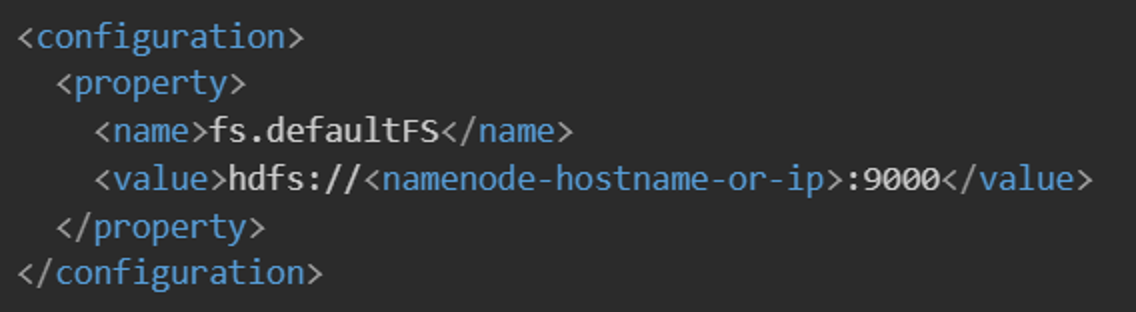
\includegraphics[width=\linewidth,height=.72\textheight,keepaspectratio]{assets/041_p013_01.png}\caption{Diagram or recorded result: Processing model and Spark abstractions.}\label{fig:041_p013_010}\end{figure}
\begin{figure}[!htbp]\centering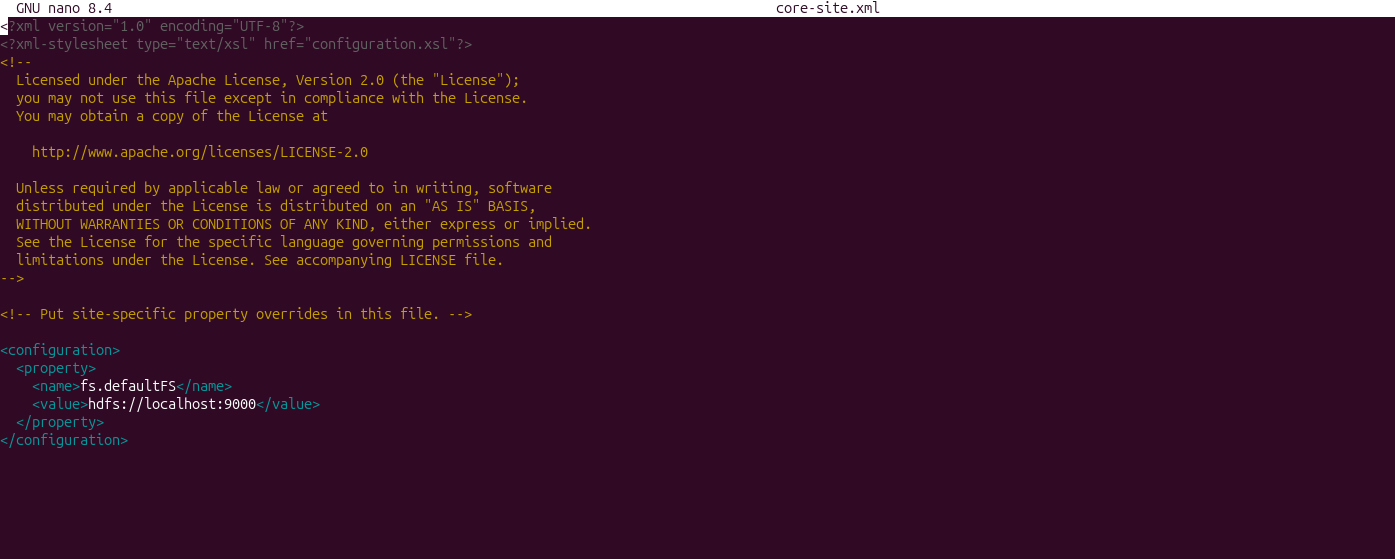
\includegraphics[width=\linewidth,height=.72\textheight,keepaspectratio]{assets/041_p013_02.png}\caption{Diagram or recorded result: Processing model and Spark abstractions.}\label{fig:041_p013_020}\end{figure}
\begin{figure}[!htbp]\centering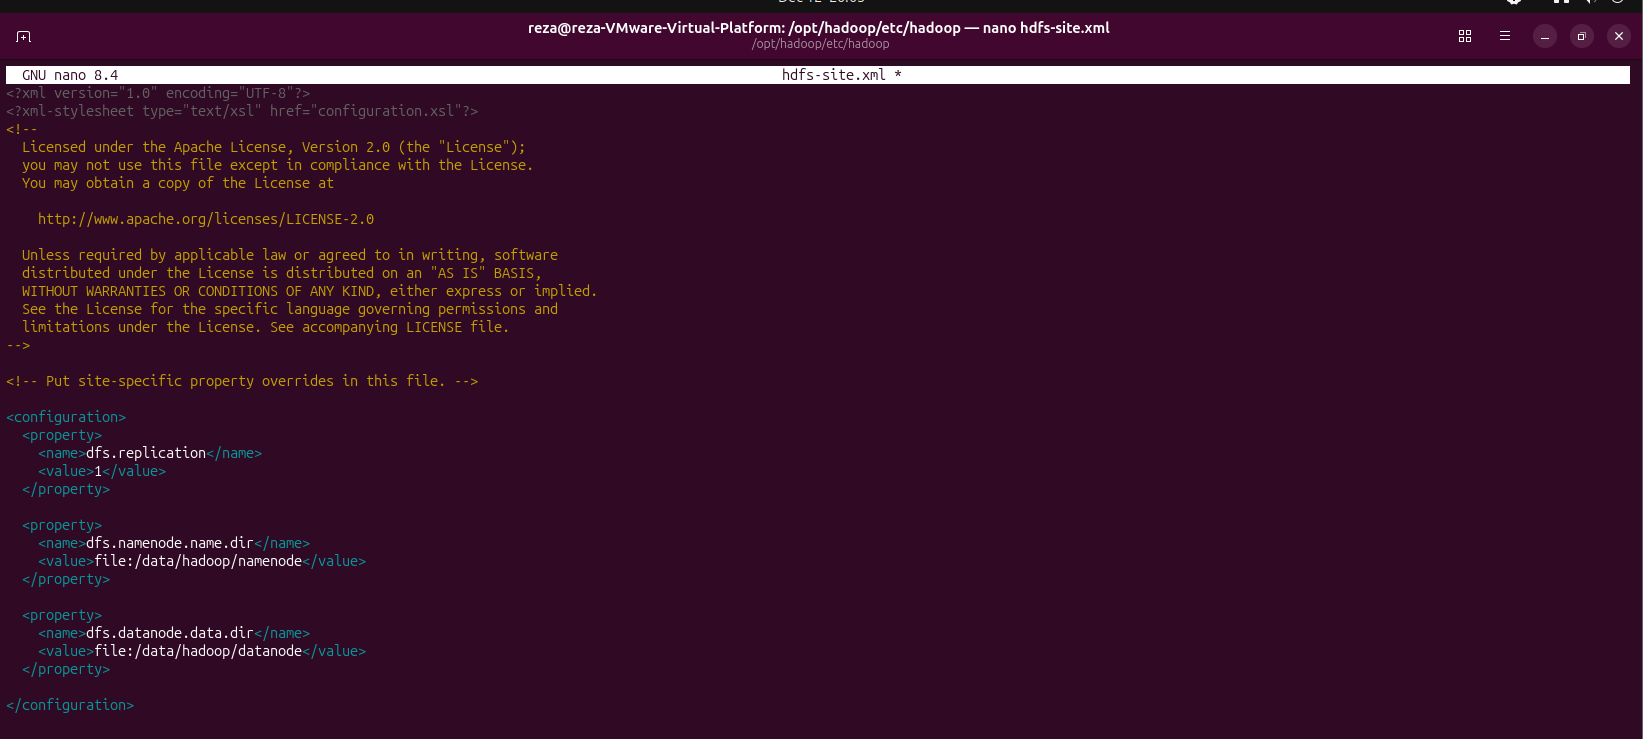
\includegraphics[width=\linewidth,height=.72\textheight,keepaspectratio]{assets/041_p014_01.png}\caption{Diagram or recorded result: Processing model and Spark abstractions.}\label{fig:041_p014_010}\end{figure}
\begin{figure}[!htbp]\centering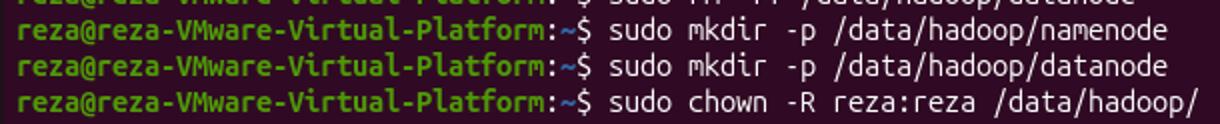
\includegraphics[width=\linewidth,height=.72\textheight,keepaspectratio]{assets/041_p014_02.png}\caption{Implementation and output: Processing model and Spark abstractions.}\label{fig:041_p014_020}\end{figure}
\clearpage
\section{Persistence, memory, and execution optimization}

Caching is useful when a dataset is reused, especially in iterative processing. MEMORY\_\allowbreak{}ONLY favors memory speed but may need recomputation when partitions do not fit. MEMORY\_\allowbreak{}AND\_\allowbreak{}DISK keeps overflow on disk. Serialized storage trades CPU overhead for a smaller representation in supported runtimes, while replicated levels retain additional copies. Python RDD objects are already serialized for storage;\allowbreak{} a serialized label does not mean a guaranteed compression ratio. RDD cache defaults and DataFrame defaults differ, so they should not be treated as one universal setting. Executor OOM may result from a large partition, skewed keys, excessive caching, oversized broadcasts, object overhead, or insufficient memory relative to concurrent tasks. Remedies include repartitioning, handling skew, reducing collected/\allowbreak{}broadcast data, unpersisting unused datasets, and adjusting resources. Increasing memory alone may leave the underlying skew unresolved. AQE uses runtime statistics to coalesce shuffle partitions, change suitable join strategies, and handle supported skewed joins. It does not optimize every operation automatically. Tungsten reduces overhead through compact representations and execution optimizations;\allowbreak{} whole-stage code generation can fuse supported operators into generated JVM code. These mechanisms do not mean that all computation becomes native machine code or that every garbage-collection cost disappears.

\begin{figure}[!htbp]\centering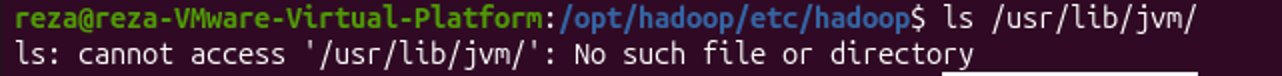
\includegraphics[width=\linewidth,height=.72\textheight,keepaspectratio]{assets/041_p015_01.png}\caption{Diagram or recorded result: Persistence, memory, and execution optimization.}\label{fig:041_p015_010}\end{figure}
\begin{figure}[!htbp]\centering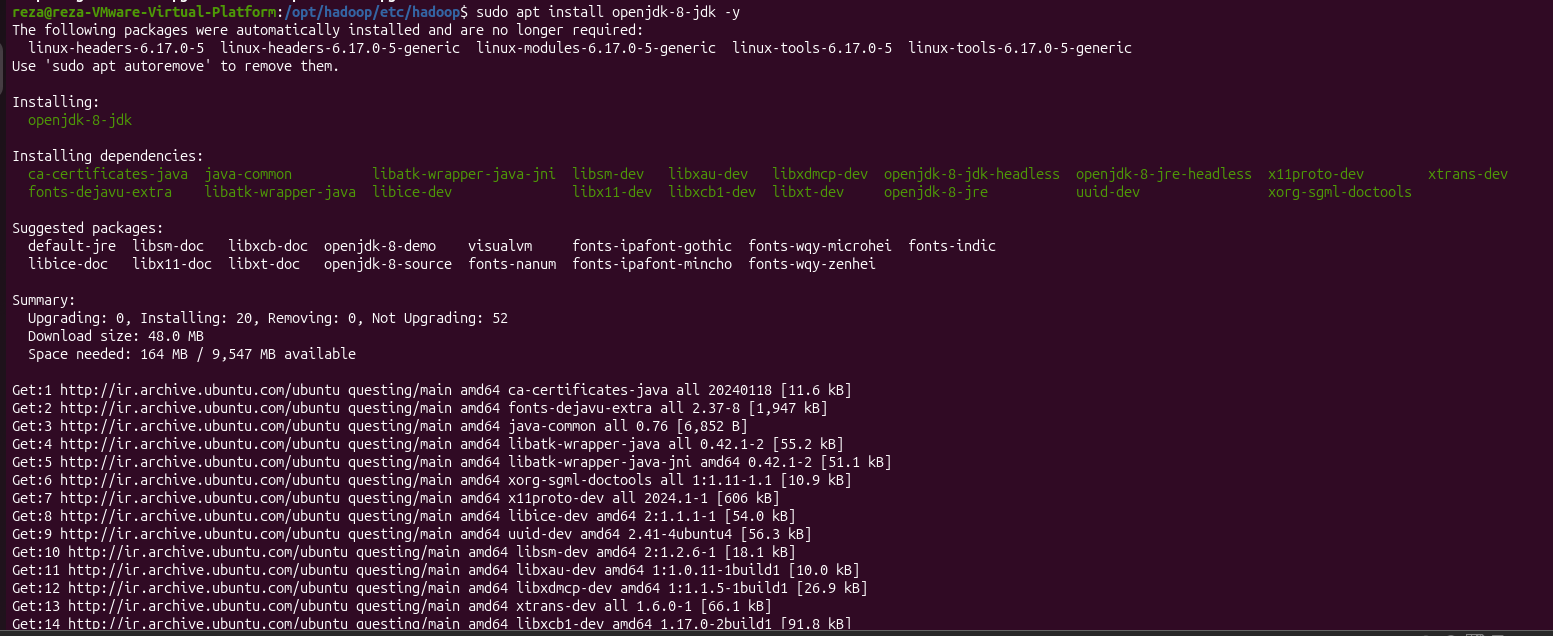
\includegraphics[width=\linewidth,height=.72\textheight,keepaspectratio]{assets/041_p015_02.png}\caption{Implementation and output: Persistence, memory, and execution optimization.}\label{fig:041_p015_020}\end{figure}
\begin{figure}[!htbp]\centering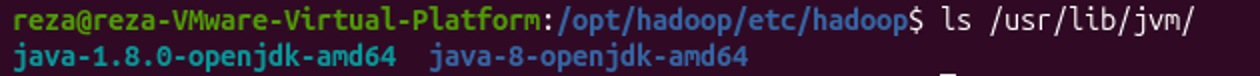
\includegraphics[width=\linewidth,height=.72\textheight,keepaspectratio]{assets/041_p015_03.png}\caption{Diagram or recorded result: Persistence, memory, and execution optimization.}\label{fig:041_p015_030}\end{figure}
\begin{figure}[!htbp]\centering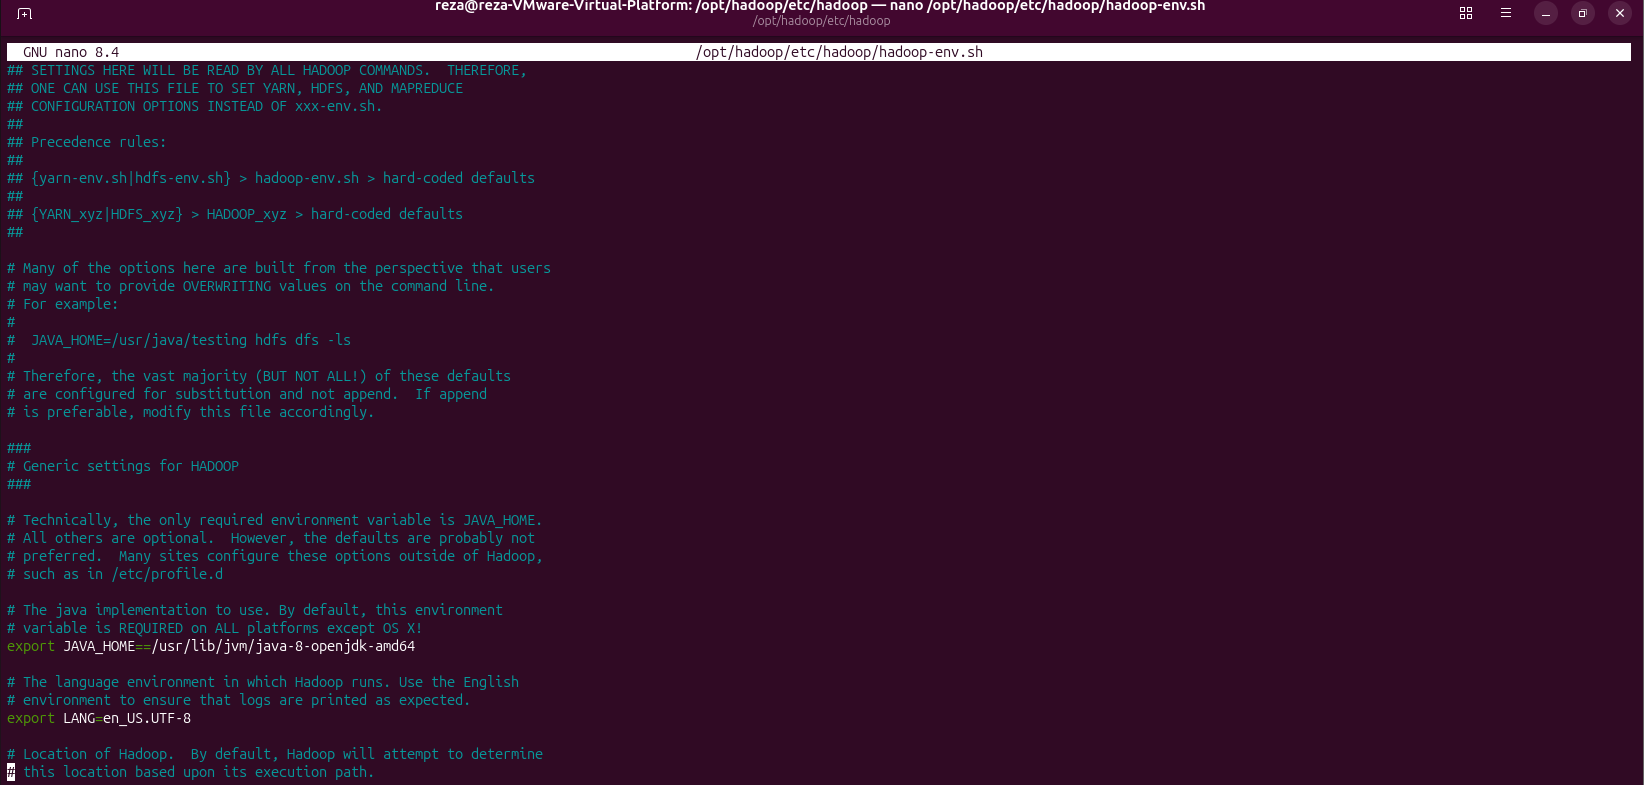
\includegraphics[width=\linewidth,height=.72\textheight,keepaspectratio]{assets/041_p016_01.png}\caption{Diagram or recorded result: Persistence, memory, and execution optimization.}\label{fig:041_p016_010}\end{figure}
\begin{figure}[!htbp]\centering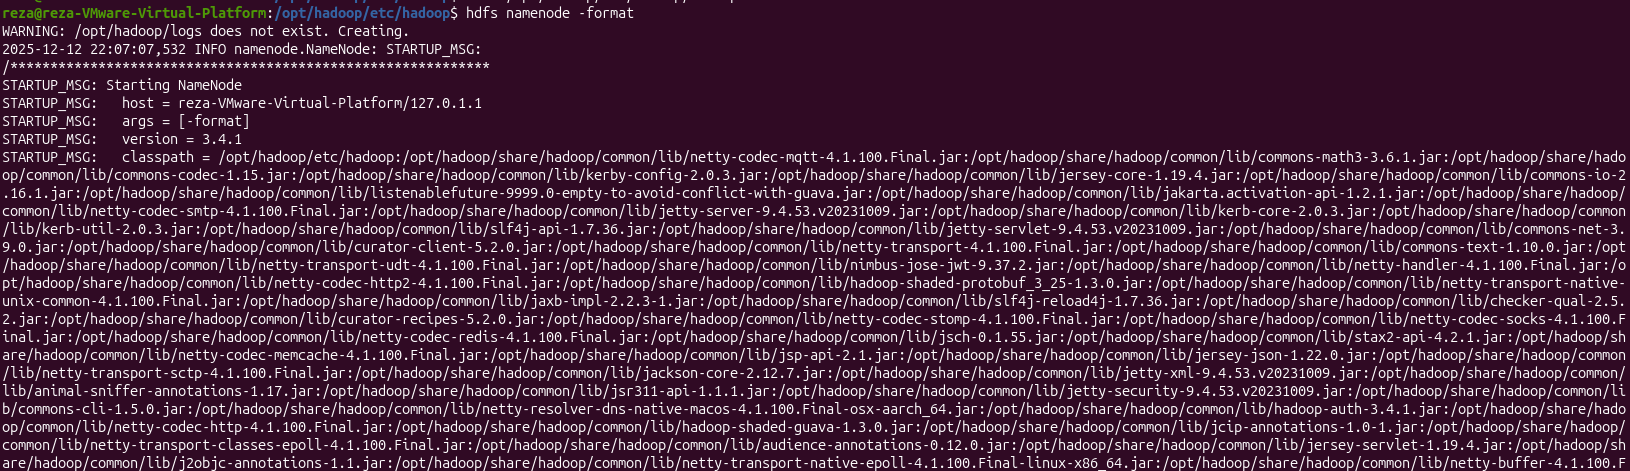
\includegraphics[width=\linewidth,height=.72\textheight,keepaspectratio]{assets/041_p016_02.png}\caption{Diagram or recorded result: Persistence, memory, and execution optimization.}\label{fig:041_p016_020}\end{figure}
\begin{figure}[!htbp]\centering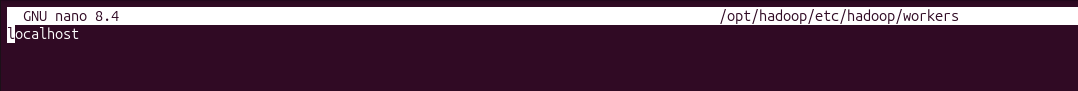
\includegraphics[width=\linewidth,height=.72\textheight,keepaspectratio]{assets/041_p016_03.png}\caption{Diagram or recorded result: Persistence, memory, and execution optimization.}\label{fig:041_p016_030}\end{figure}
\clearpage
\section{Deployment, file formats, and resource sharing}

Standalone is suitable for a dedicated, relatively simple Spark cluster. YARN integrates with an existing Hadoop resource environment. Kubernetes offers container-oriented scheduling, but requires operational configuration for resources, storage, networking, and security. No deployment mode provides correct scaling or security merely by being selected. Parquet and ORC support column pruning, compression, and statistics-based data skipping;\allowbreak{} they are especially useful when reading selected columns from large analytical datasets. Delta Lake adds transactional table management and historical versions, subject to retained logs/\allowbreak{}data. Z-ordering can improve data locality and skipping;\allowbreak{} it is not an authorization mechanism. Warehouse versus lakehouse selection depends on governance, workload, infrastructure, and cost rather than a strict old-versus-new distinction. FIFO and Fair scheduling concern jobs sharing a Spark context;\allowbreak{} cluster-manager allocation between applications is a separate layer. Fair pools can specify weights and minimum shares. Tasks already running are normally not preempted simply because another pool submits work. Pool properties must be set in the appropriate submitting thread. Dynamic allocation requests or releases executors according to workload and configured limits;\allowbreak{} it requires a compatible way to preserve shuffle data and is not an instantaneous fairness guarantee.

\begin{figure}[!htbp]\centering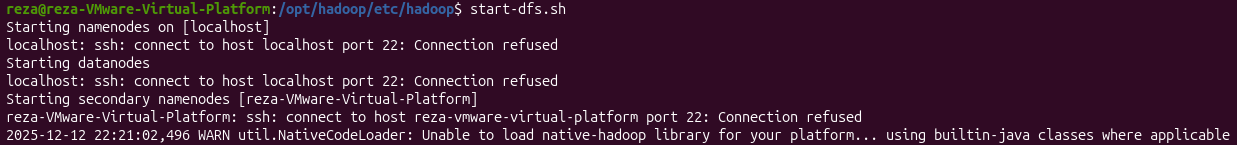
\includegraphics[width=\linewidth,height=.72\textheight,keepaspectratio]{assets/041_p017_01.png}\caption{Diagram or recorded result: Deployment, file formats, and resource sharing.}\label{fig:041_p017_010}\end{figure}
\begin{figure}[!htbp]\centering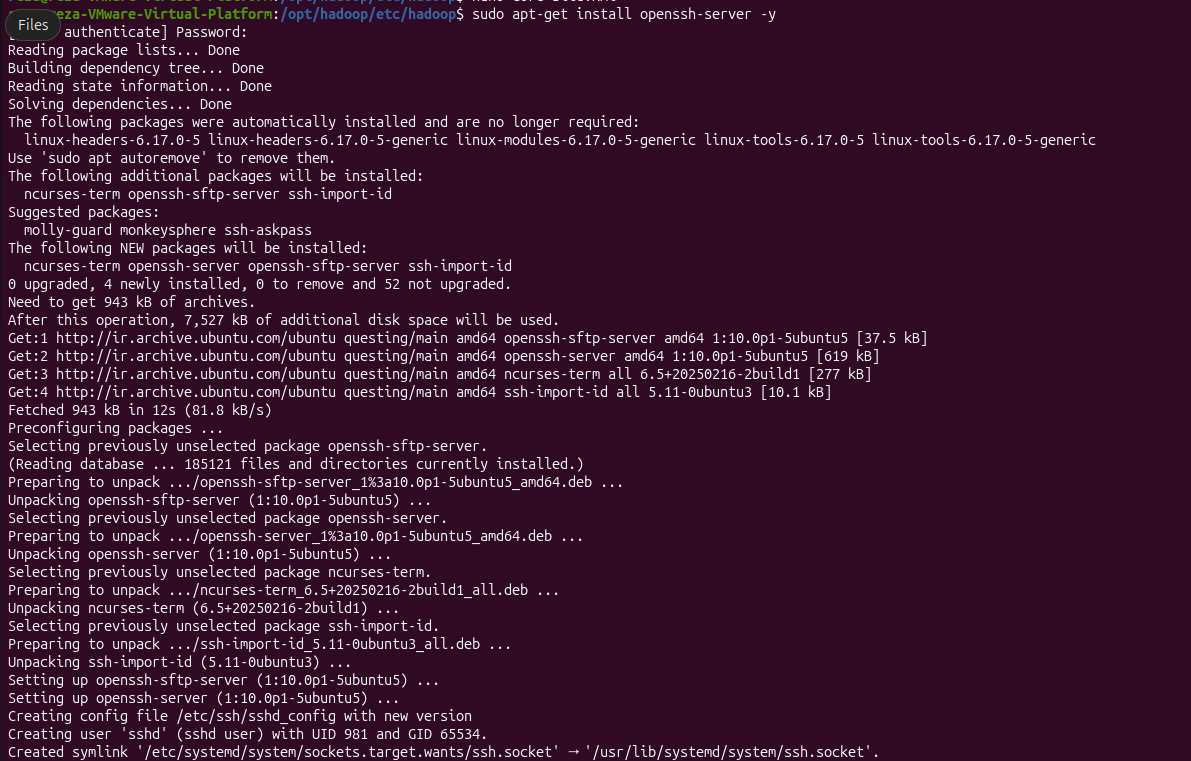
\includegraphics[width=\linewidth,height=.72\textheight,keepaspectratio]{assets/041_p017_02.png}\caption{Implementation and output: Deployment, file formats, and resource sharing.}\label{fig:041_p017_020}\end{figure}
\begin{figure}[!htbp]\centering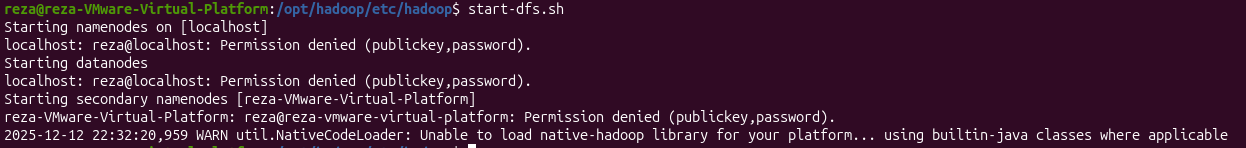
\includegraphics[width=\linewidth,height=.72\textheight,keepaspectratio]{assets/041_p018_01.png}\caption{Diagram or recorded result: Deployment, file formats, and resource sharing.}\label{fig:041_p018_010}\end{figure}
\begin{figure}[!htbp]\centering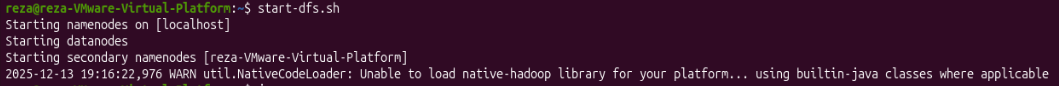
\includegraphics[width=\linewidth,height=.72\textheight,keepaspectratio]{assets/041_p018_02.png}\caption{Diagram or recorded result: Deployment, file formats, and resource sharing.}\label{fig:041_p018_020}\end{figure}
\clearpage
\section{Part A: installing and configuring Hadoop}

The supplied installation record follows hadoop\_\allowbreak{}installation.md. Hadoop 3.4.1 was downloaded, extracted, and placed under /\allowbreak{}opt/\allowbreak{}hadoop. Environment variables were added to \textasciitilde{}/\allowbreak{}.bashrc. Linux paths are case-sensitive. Use the actual /\allowbreak{}opt/\allowbreak{}hadoop and /\allowbreak{}data/\allowbreak{}hadoop directories consistently in commands and configuration. Moving files under /\allowbreak{}opt and configuring protected directories requires appropriate ownership or sudo. The core configuration sets fs.defaultFS to hdfs:\allowbreak{}/\allowbreak{}/\allowbreak{}localhost:\allowbreak{}9000. The HDFS configuration uses replication=\allowbreak{}1 for the single-machine laboratory and separate NameNode/\allowbreak{}DataNode directories under /\allowbreak{}data/\allowbreak{}hadoop. Directory ownership must permit the Hadoop account to access them. JAVA\_\allowbreak{}HOME was configured for the Java installation used by Hadoop. The source describes Java 8 for this stage and Java 11 for a later Spark stage;\allowbreak{} each component's environment must be checked explicitly rather than assuming one shell value works for all services. After configuring the worker as localhost, the new NameNode was formatted once. The first start-dfs.sh attempt failed because an SSH service was absent. Installing openssh-server addressed that problem. A later passwordless-SSH failure was addressed by generating a local key and adding its public key to authorized\_\allowbreak{}keys. Existing keys should be retained rather than overwritten when adapting the procedure. Once SSH access was configured, start-dfs.sh launched the services and hdfs dfsadmin -report displayed the DataNode status and capacity.

\begin{figure}[!htbp]\centering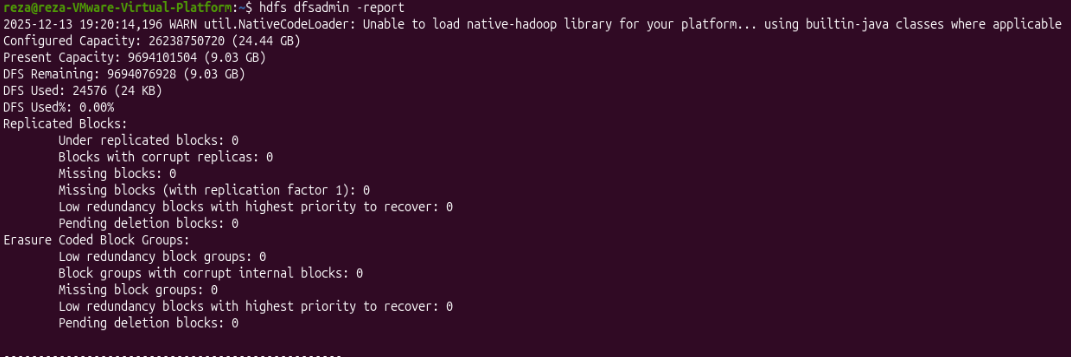
\includegraphics[width=\linewidth,height=.72\textheight,keepaspectratio]{assets/041_p019_01.png}\caption{Diagram or recorded result: Part A: installing and configuring Hadoop.}\label{fig:041_p019_010}\end{figure}
\begin{figure}[!htbp]\centering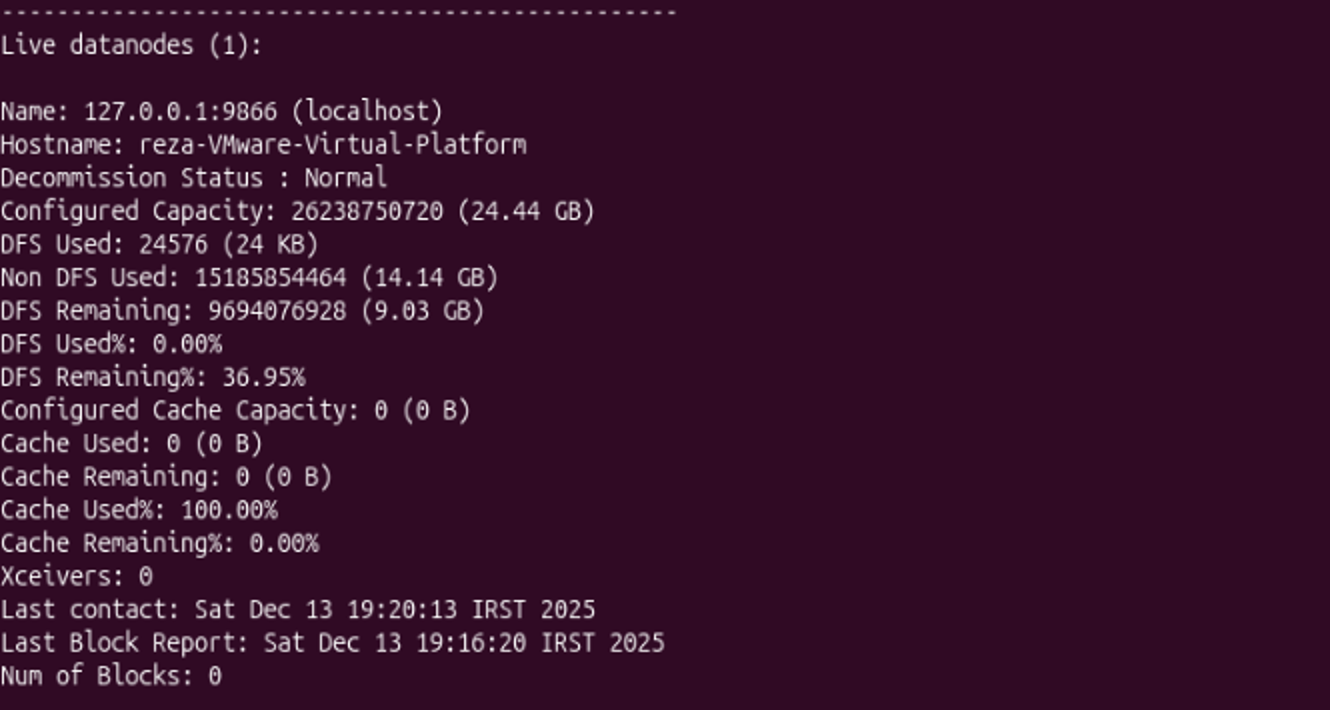
\includegraphics[width=\linewidth,height=.72\textheight,keepaspectratio]{assets/041_p019_02.png}\caption{Diagram or recorded result: Part A: installing and configuring Hadoop.}\label{fig:041_p019_020}\end{figure}
\begin{figure}[!htbp]\centering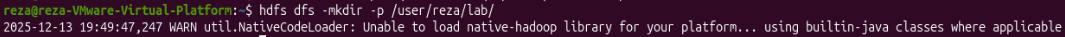
\includegraphics[width=\linewidth,height=.72\textheight,keepaspectratio]{assets/041_p019_03.png}\caption{Diagram or recorded result: Part A: installing and configuring Hadoop.}\label{fig:041_p019_030}\end{figure}
\begin{figure}[!htbp]\centering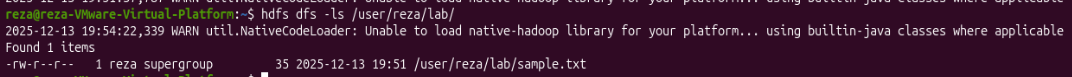
\includegraphics[width=\linewidth,height=.72\textheight,keepaspectratio]{assets/041_p020_01.png}\caption{Diagram or recorded result: Part A: installing and configuring Hadoop.}\label{fig:041_p020_010}\end{figure}
\begin{figure}[!htbp]\centering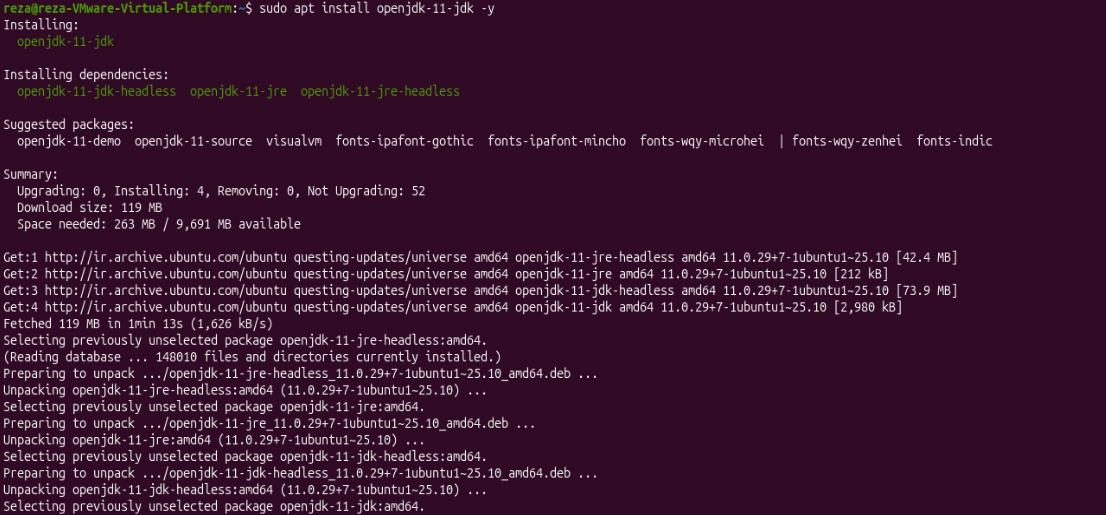
\includegraphics[width=\linewidth,height=.72\textheight,keepaspectratio]{assets/041_p021_02.png}\caption{Implementation and output: Part A: installing and configuring Hadoop.}\label{fig:041_p021_020}\end{figure}
\begin{figure}[!htbp]\centering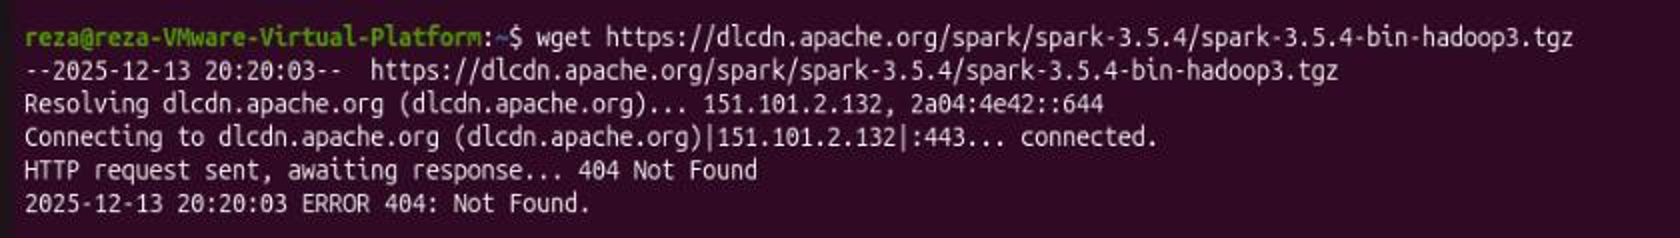
\includegraphics[width=\linewidth,height=.72\textheight,keepaspectratio]{assets/041_p021_03.png}\caption{Implementation and output: Part A: installing and configuring Hadoop.}\label{fig:041_p021_030}\end{figure}
\begin{figure}[!htbp]\centering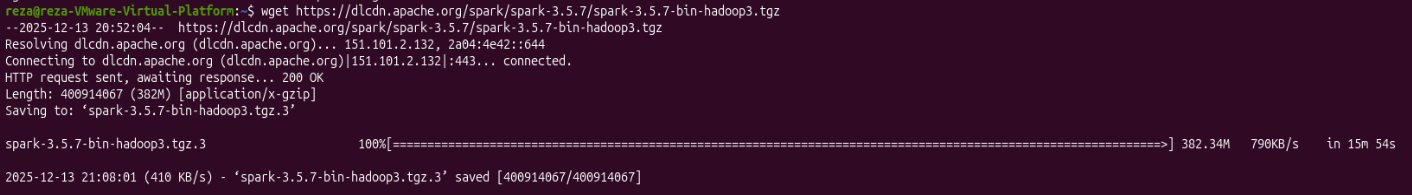
\includegraphics[width=\linewidth,height=.72\textheight,keepaspectratio]{assets/041_p022_01.png}\caption{Implementation and output: Part A: installing and configuring Hadoop.}\label{fig:041_p022_010}\end{figure}
\begin{figure}[!htbp]\centering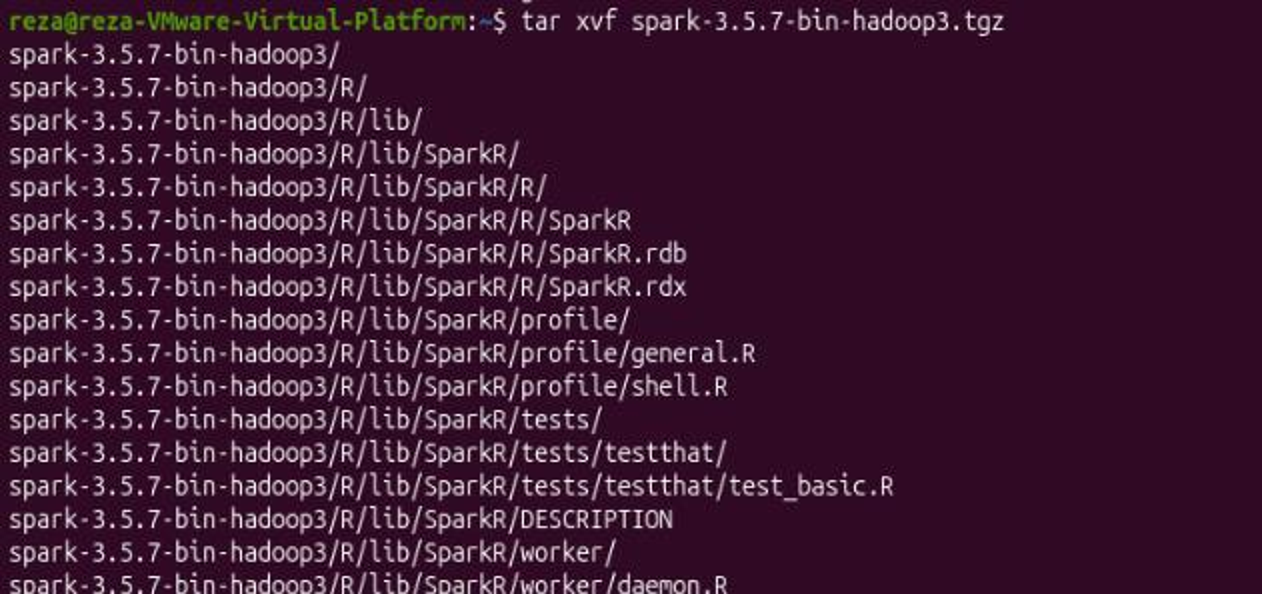
\includegraphics[width=\linewidth,height=.72\textheight,keepaspectratio]{assets/041_p022_02.png}\caption{Implementation and output: Part A: installing and configuring Hadoop.}\label{fig:041_p022_020}\end{figure}
\begin{figure}[!htbp]\centering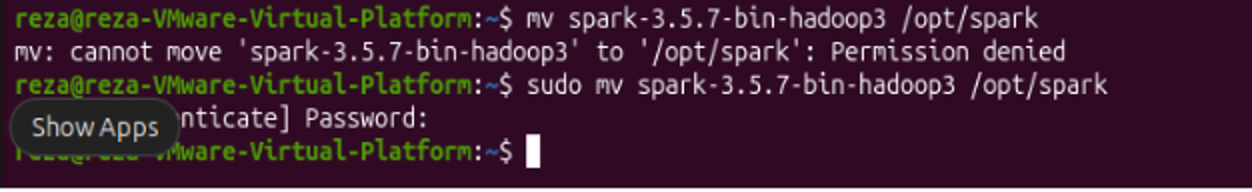
\includegraphics[width=\linewidth,height=.72\textheight,keepaspectratio]{assets/041_p022_03.png}\caption{Implementation and output: Part A: installing and configuring Hadoop.}\label{fig:041_p022_030}\end{figure}
\begin{figure}[!htbp]\centering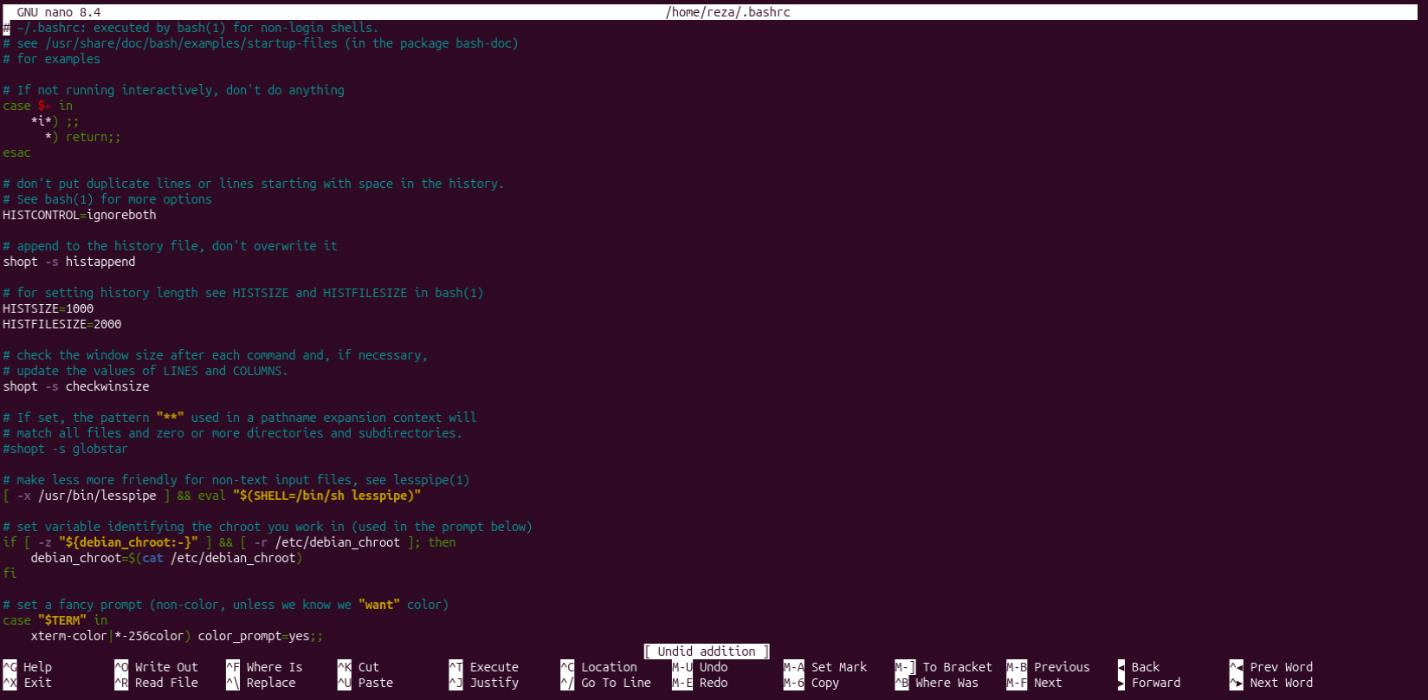
\includegraphics[width=\linewidth,height=.72\textheight,keepaspectratio]{assets/041_p023_01.png}\caption{Diagram or recorded result: Part A: installing and configuring Hadoop.}\label{fig:041_p023_010}\end{figure}
\begin{figure}[!htbp]\centering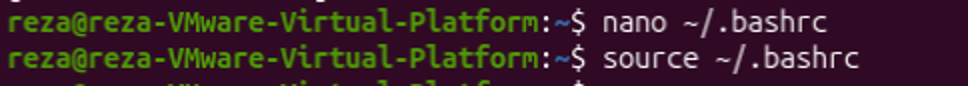
\includegraphics[width=\linewidth,height=.72\textheight,keepaspectratio]{assets/041_p023_02.png}\caption{Diagram or recorded result: Part A: installing and configuring Hadoop.}\label{fig:041_p023_020}\end{figure}
\begin{figure}[!htbp]\centering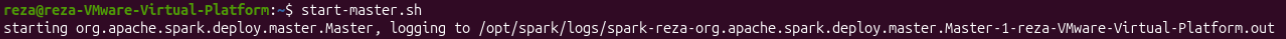
\includegraphics[width=\linewidth,height=.72\textheight,keepaspectratio]{assets/041_p023_03.png}\caption{Implementation and output: Part A: installing and configuring Hadoop.}\label{fig:041_p023_030}\end{figure}
\begin{figure}[!htbp]\centering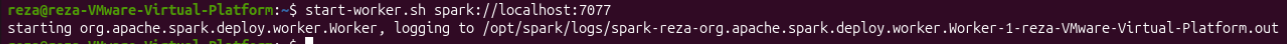
\includegraphics[width=\linewidth,height=.72\textheight,keepaspectratio]{assets/041_p023_04.png}\caption{Implementation and output: Part A: installing and configuring Hadoop.}\label{fig:041_p023_040}\end{figure}
\begin{figure}[!htbp]\centering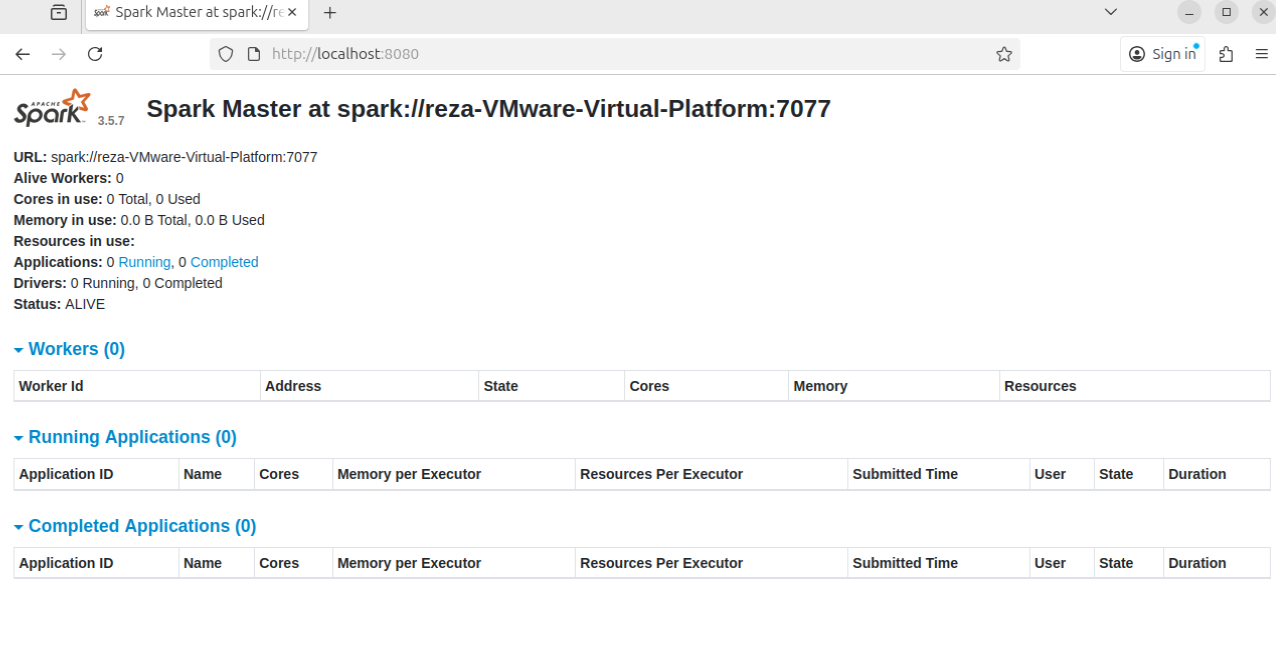
\includegraphics[width=\linewidth,height=.72\textheight,keepaspectratio]{assets/041_p024_01.png}\caption{Implementation and output: Part A: installing and configuring Hadoop.}\label{fig:041_p024_010}\end{figure}
\begin{figure}[!htbp]\centering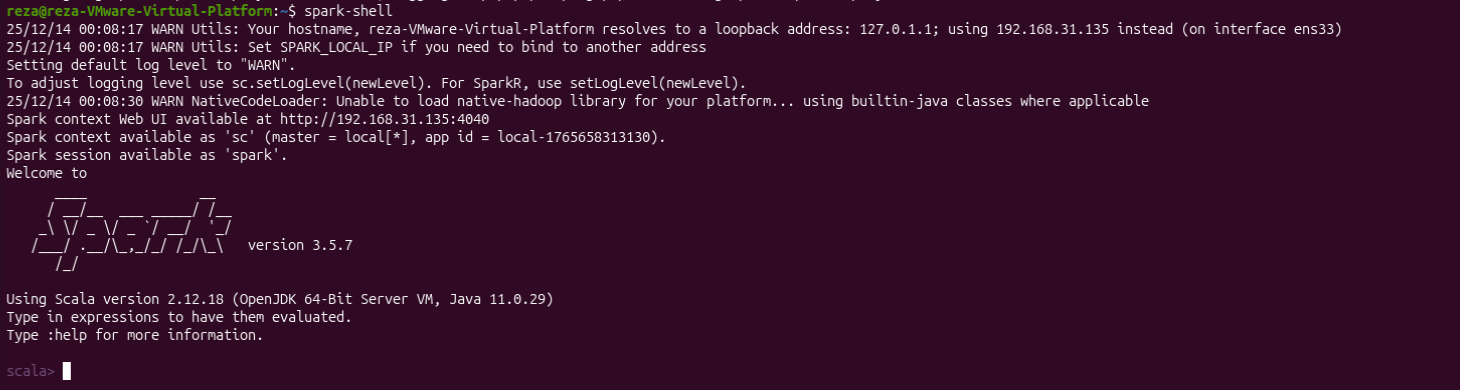
\includegraphics[width=\linewidth,height=.72\textheight,keepaspectratio]{assets/041_p024_02.png}\caption{Implementation and output: Part A: installing and configuring Hadoop.}\label{fig:041_p024_020}\end{figure}
\begin{figure}[!htbp]\centering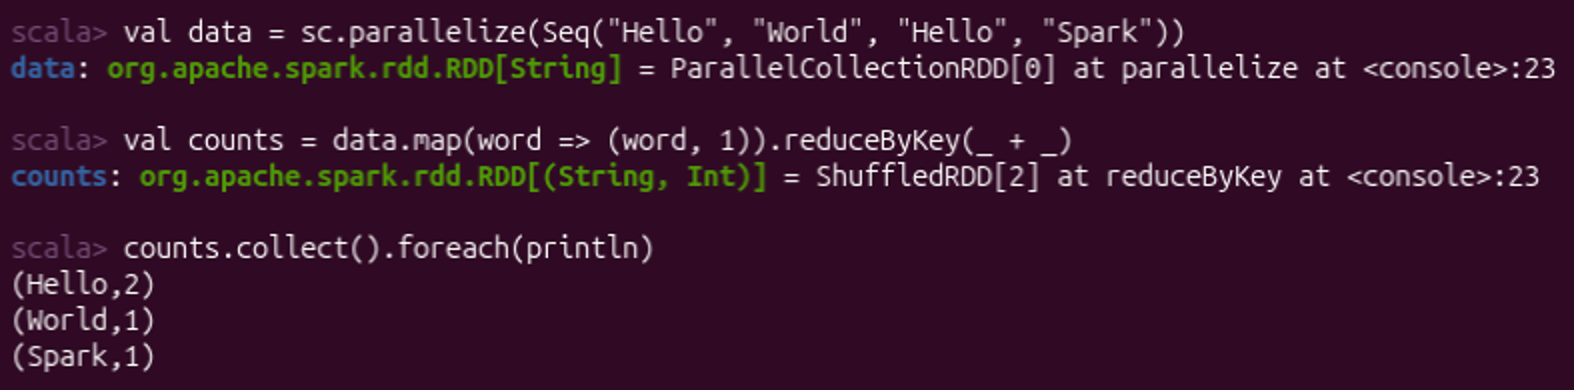
\includegraphics[width=\linewidth,height=.72\textheight,keepaspectratio]{assets/041_p025_01.png}\caption{Implementation and output: Part A: installing and configuring Hadoop.}\label{fig:041_p025_010}\end{figure}
\begin{figure}[!htbp]\centering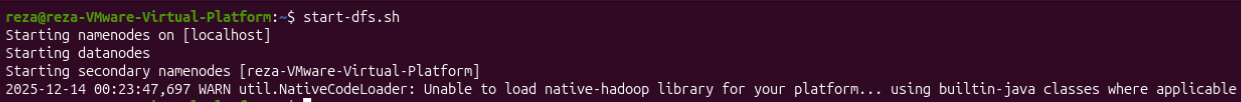
\includegraphics[width=\linewidth,height=.72\textheight,keepaspectratio]{assets/041_p025_02.png}\caption{Diagram or recorded result: Part A: installing and configuring Hadoop.}\label{fig:041_p025_020}\end{figure}
\begin{figure}[!htbp]\centering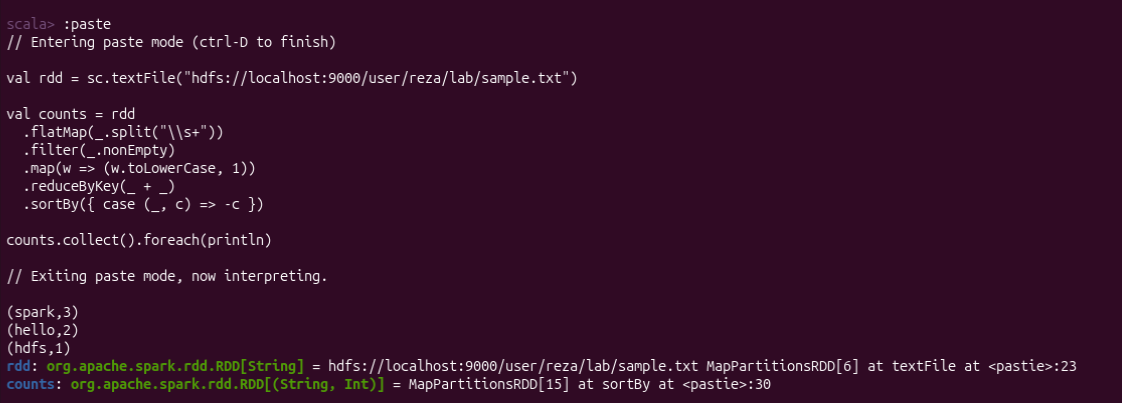
\includegraphics[width=\linewidth,height=.72\textheight,keepaspectratio]{assets/041_p025_03.png}\caption{Implementation and output: Part A: installing and configuring Hadoop.}\label{fig:041_p025_030}\end{figure}
\begin{figure}[!htbp]\centering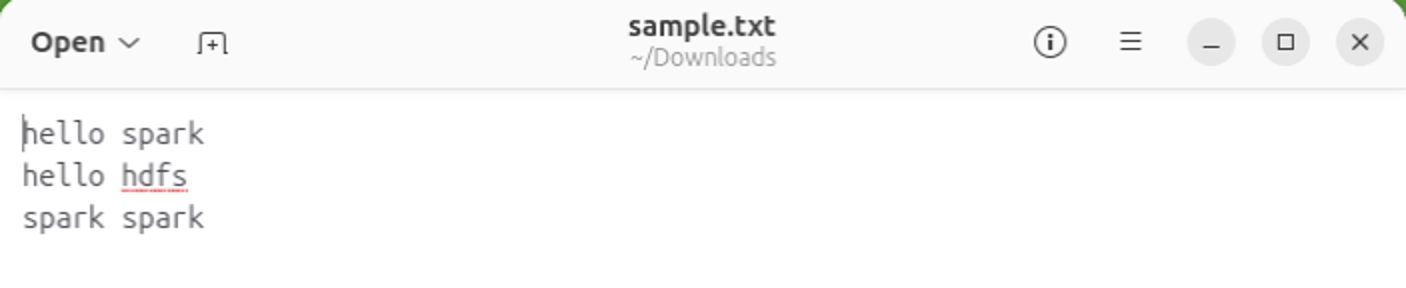
\includegraphics[width=\linewidth,height=.72\textheight,keepaspectratio]{assets/041_p025_04.png}\caption{Implementation and output: Part A: installing and configuring Hadoop.}\label{fig:041_p025_040}\end{figure}
\clearpage
\section{HDFS upload test}

The report creates sample.txt containing three lines, creates /\allowbreak{}user/\allowbreak{}reza/\allowbreak{}lab/\allowbreak{}, uploads the file, and lists the directory. The listing confirms that sample.txt appears in HDFS. This is a functional upload/\allowbreak{}listing test;\allowbreak{} it does not establish replication across machines because the documented topology has one DataNode.

\begin{figure}[!htbp]\centering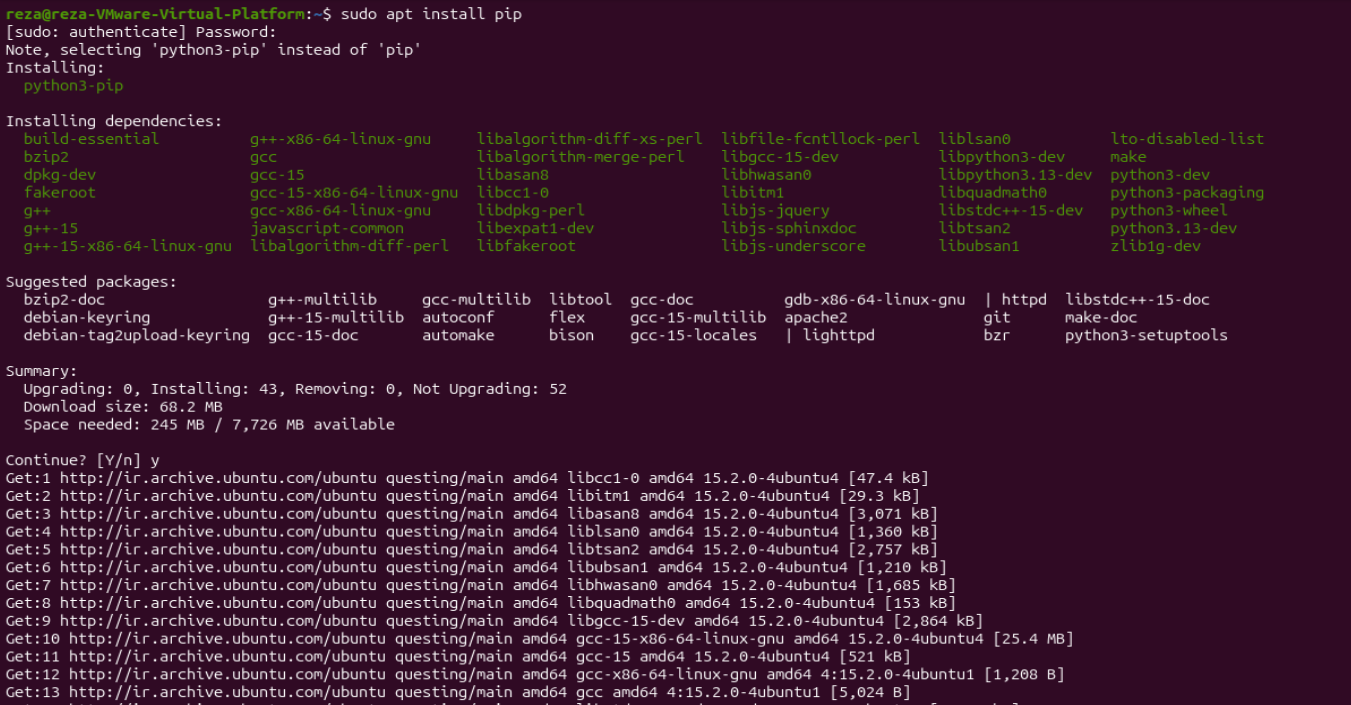
\includegraphics[width=\linewidth,height=.72\textheight,keepaspectratio]{assets/041_p026_01.png}\caption{Implementation and output: HDFS upload test.}\label{fig:041_p026_010}\end{figure}
\begin{figure}[!htbp]\centering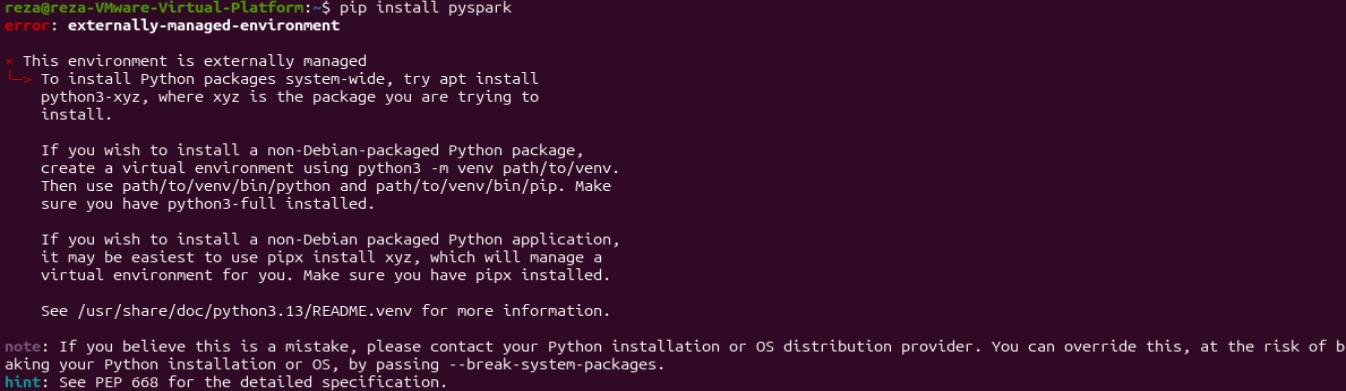
\includegraphics[width=\linewidth,height=.72\textheight,keepaspectratio]{assets/041_p026_02.png}\caption{Implementation and output: HDFS upload test.}\label{fig:041_p026_020}\end{figure}
\clearpage
\section{Part B: Spark installation and shell tests}

The Spark guide initially referred to version 3.5.4. A download attempt failed, and the report switched to Spark 3.5.7. All subsequent extraction paths and example JAR names must therefore use 3.5.7 consistently. SPARK\_\allowbreak{}HOME and PATH were added to \textasciitilde{}/\allowbreak{}.bashrc. start-master.sh launched the master and start-worker.sh spark:\allowbreak{}/\allowbreak{}/\allowbreak{}localhost:\allowbreak{}7077 registered the worker. The browser interface on port 8080 showed the deployment. A Scala shell counted the list Hello, World, Hello, Spark. A further Scala test loaded sample.txt from HDFS and applied flatMap, filter, map, reduceByKey, and sorting. The correct sample counts are spark=\allowbreak{}3, hello=\allowbreak{}2, hdfs=\allowbreak{}1.

\begin{figure}[!htbp]\centering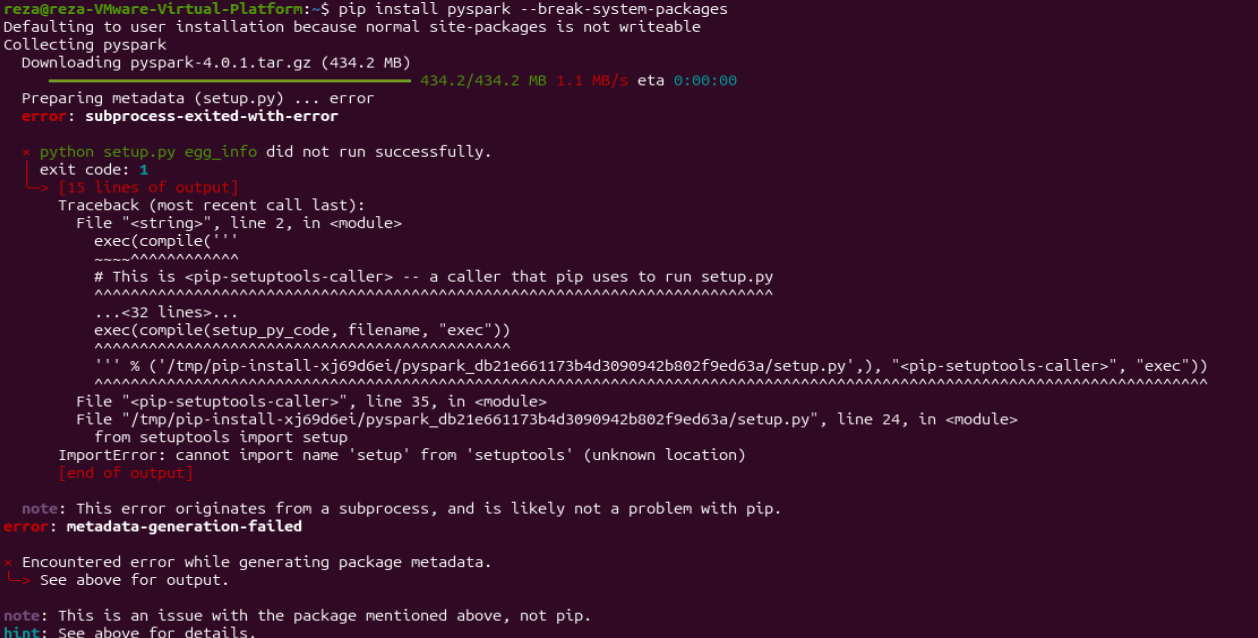
\includegraphics[width=\linewidth,height=.72\textheight,keepaspectratio]{assets/041_p027_01.png}\caption{Implementation and output: Part B: Spark installation and shell tests.}\label{fig:041_p027_010}\end{figure}
\begin{figure}[!htbp]\centering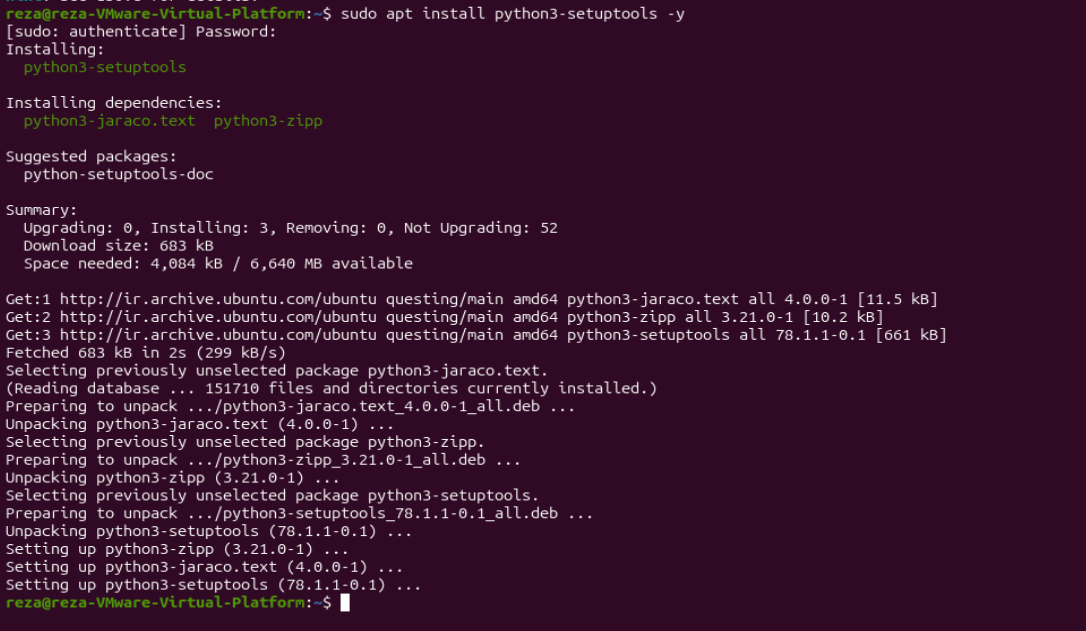
\includegraphics[width=\linewidth,height=.72\textheight,keepaspectratio]{assets/041_p027_02.png}\caption{Implementation and output: Part B: Spark installation and shell tests.}\label{fig:041_p027_020}\end{figure}
\begin{figure}[!htbp]\centering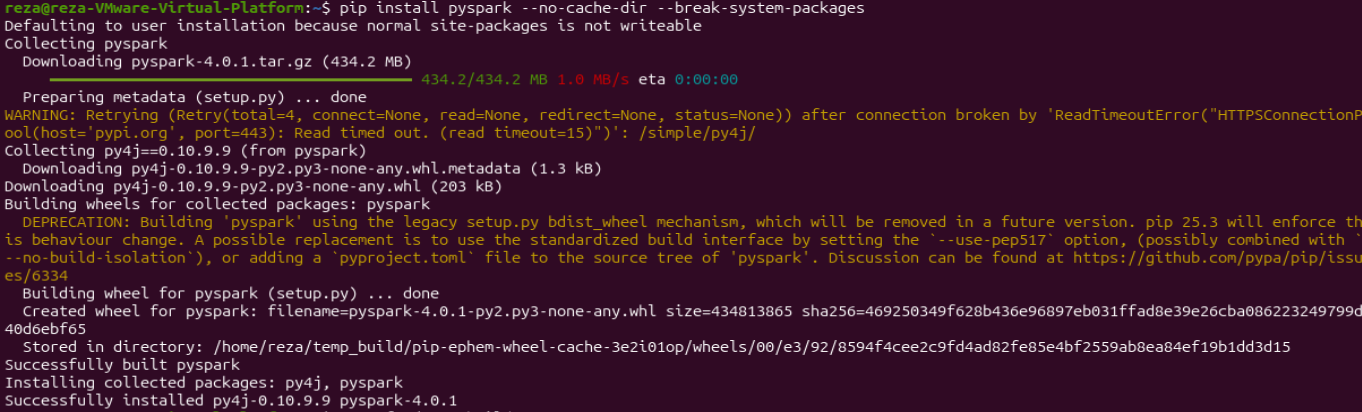
\includegraphics[width=\linewidth,height=.72\textheight,keepaspectratio]{assets/041_p028_01.png}\caption{Implementation and output: Part B: Spark installation and shell tests.}\label{fig:041_p028_010}\end{figure}
\begin{figure}[!htbp]\centering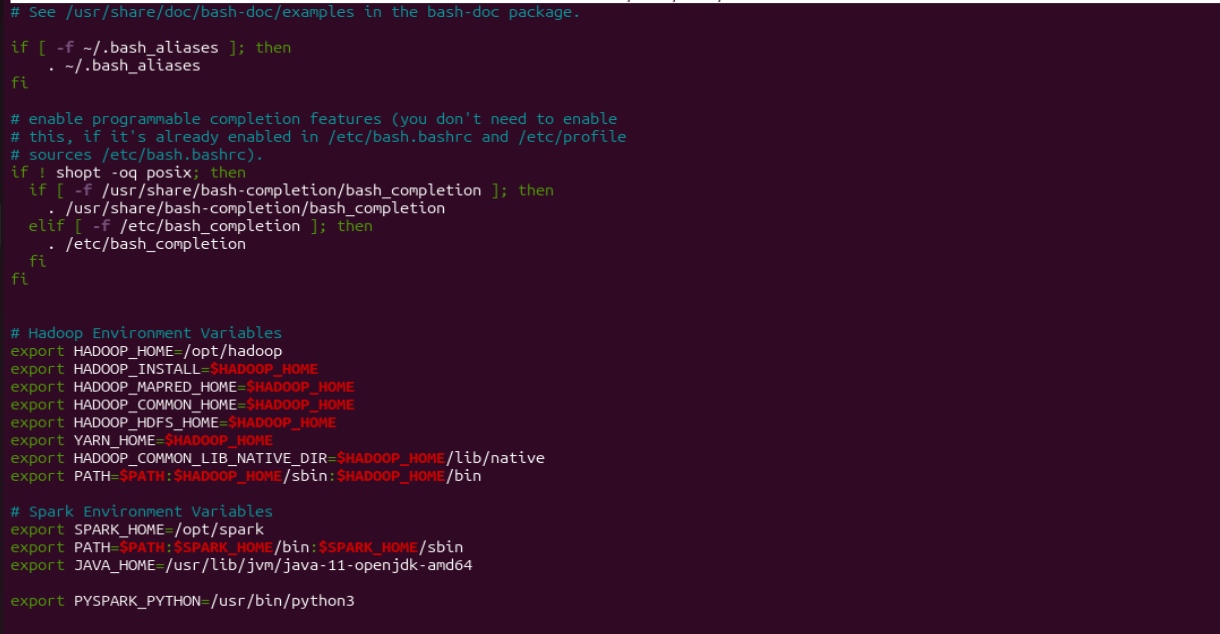
\includegraphics[width=\linewidth,height=.72\textheight,keepaspectratio]{assets/041_p028_02.png}\caption{Implementation and output: Part B: Spark installation and shell tests.}\label{fig:041_p028_020}\end{figure}
\clearpage
\section{Python environment troubleshooting}

The initial global pip installation was refused because the operating system manages that Python environment. The submission used --break-system-packages after installing setuptools. For a reproducible setup, use an isolated environment and a matching PySpark version instead of modifying the managed interpreter:\allowbreak{}


\begin{quote}\small\ttfamily\raggedright
python3 -m venv .venv\par
source .venv/\allowbreak{}bin/\allowbreak{}activate\par
python -m pip install --upgrade pip setuptools\par
python -m pip install pyspark=\allowbreak{}=\allowbreak{}3.5.7\par\end{quote}

The reported PySpark shell test parallelizes [1,2,3,4,5], squares each entry, and prints [1,4,9,16,25]. That confirms the basic Python-to-Spark computation for the tested environment.

\begin{figure}[!htbp]\centering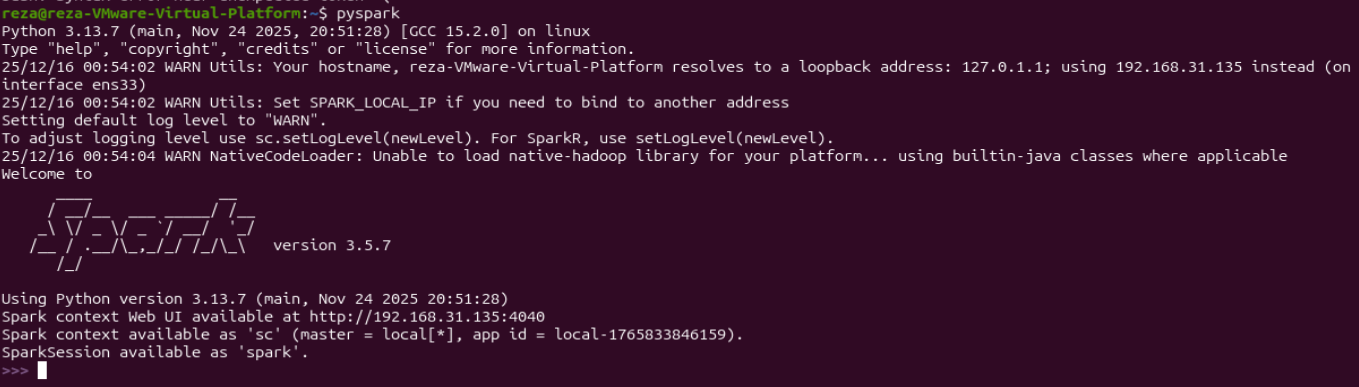
\includegraphics[width=\linewidth,height=.72\textheight,keepaspectratio]{assets/041_p029_01.png}\caption{Implementation and output: Python environment troubleshooting.}\label{fig:041_p029_010}\end{figure}
\begin{figure}[!htbp]\centering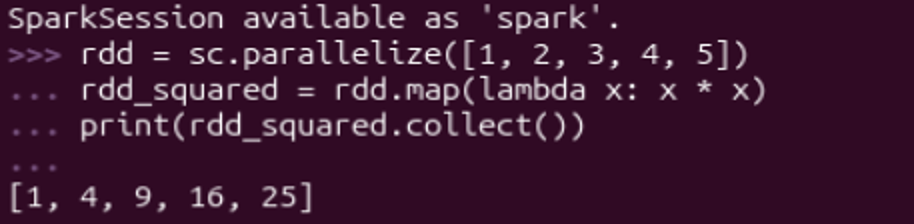
\includegraphics[width=\linewidth,height=.72\textheight,keepaspectratio]{assets/041_p029_02.png}\caption{Implementation and output: Python environment troubleshooting.}\label{fig:041_p029_020}\end{figure}
\begin{figure}[!htbp]\centering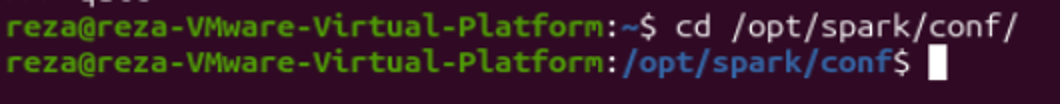
\includegraphics[width=\linewidth,height=.72\textheight,keepaspectratio]{assets/041_p029_03.png}\caption{Implementation and output: Python environment troubleshooting.}\label{fig:041_p029_030}\end{figure}
\begin{figure}[!htbp]\centering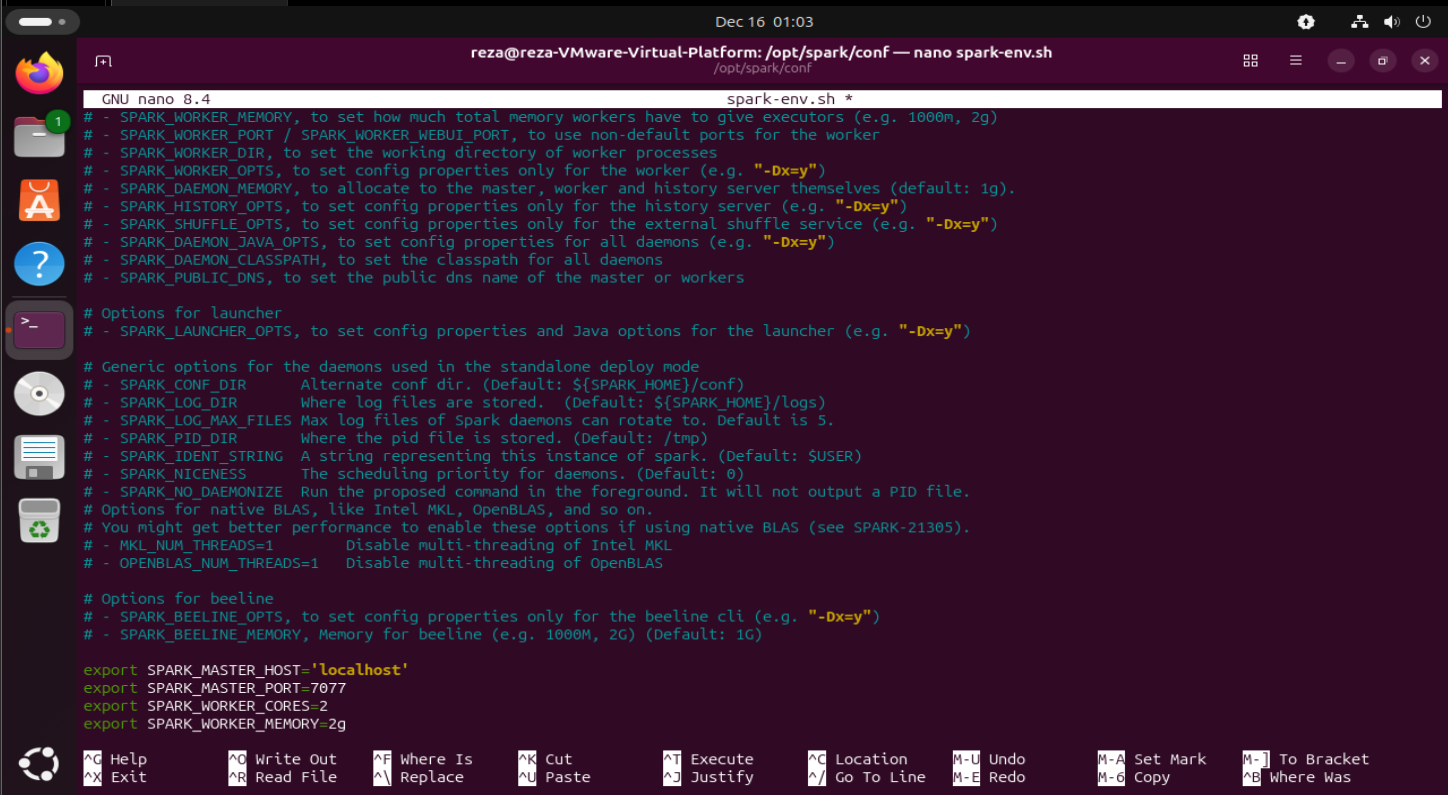
\includegraphics[width=\linewidth,height=.72\textheight,keepaspectratio]{assets/041_p030_01.png}\caption{Implementation and output: Python environment troubleshooting.}\label{fig:041_p030_010}\end{figure}
\clearpage
\section{Master/worker configuration and final integration}

spark-env.sh and workers were created from their templates. The workers file contains localhost because the master and worker share one machine. A hosts entry maps master to the local address. The master UI on port 8080, worker UI on port 8081, and the master's JSON endpoint were used for inspection. spark-defaults.conf sets spark.master to spark:\allowbreak{}/\allowbreak{}/\allowbreak{}master:\allowbreak{}7077 and a local driver address. SPARK\_\allowbreak{}LOCAL\_\allowbreak{}IP=\allowbreak{}127.0.0.1 is appropriate only to this single-host example;\allowbreak{} a multi-host deployment needs reachable addresses. The final SparkPi example requests 1 GB for the driver and executor and uses 10 samples/\allowbreak{}partitions as stated by the example invocation. The source reports Pi is roughly 3.1406631406631407. The consistent command for the installed version is:\allowbreak{}


\begin{quote}\small\ttfamily\raggedright
spark-submit --class org.apache.spark.examples.SparkPi \textbackslash{}\par
 --master spark:\allowbreak{}/\allowbreak{}/\allowbreak{}master:\allowbreak{}7077 --executor-memory 1G \textbackslash{}\par
 --driver-memory 1G \textbackslash{}\par
 /\allowbreak{}opt/\allowbreak{}spark/\allowbreak{}examples/\allowbreak{}jars/\allowbreak{}spark-examples\_\allowbreak{}2.12-3.5.7.jar 10\par\end{quote}

The installation evidence supports a working classroom HDFS/\allowbreak{}Spark integration on the documented host. It does not establish multi-node throughput, fault tolerance, authentication, or production readiness. All deployment screenshots and the full troubleshooting sequence are retained.

\begin{figure}[!htbp]\centering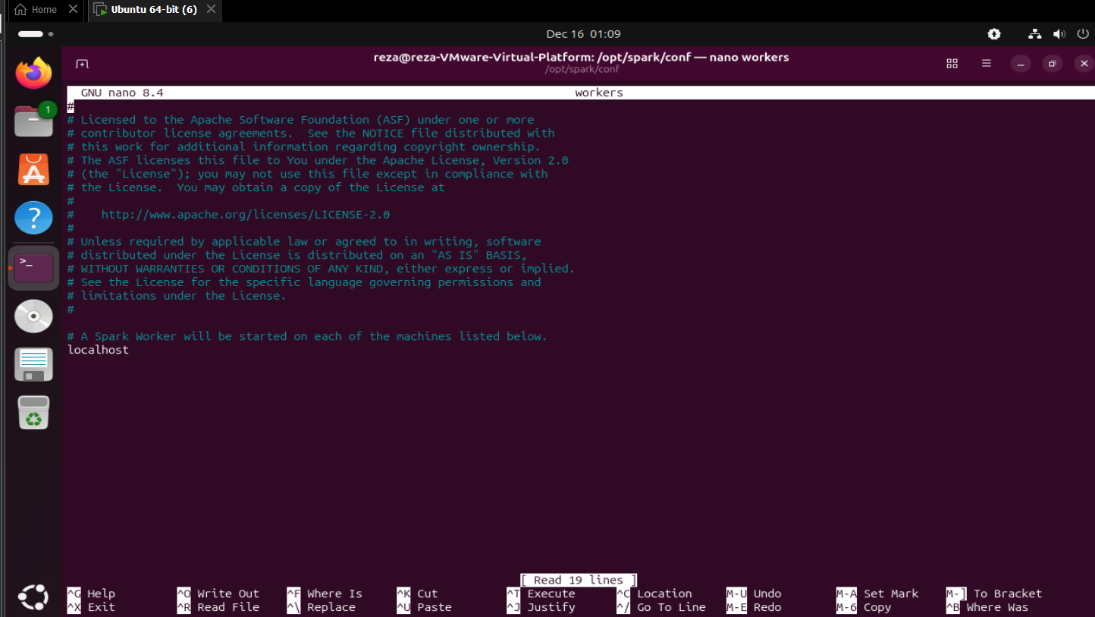
\includegraphics[width=\linewidth,height=.72\textheight,keepaspectratio]{assets/041_p031_01.png}\caption{Implementation and output: Master/worker configuration and final integration.}\label{fig:041_p031_010}\end{figure}
\begin{figure}[!htbp]\centering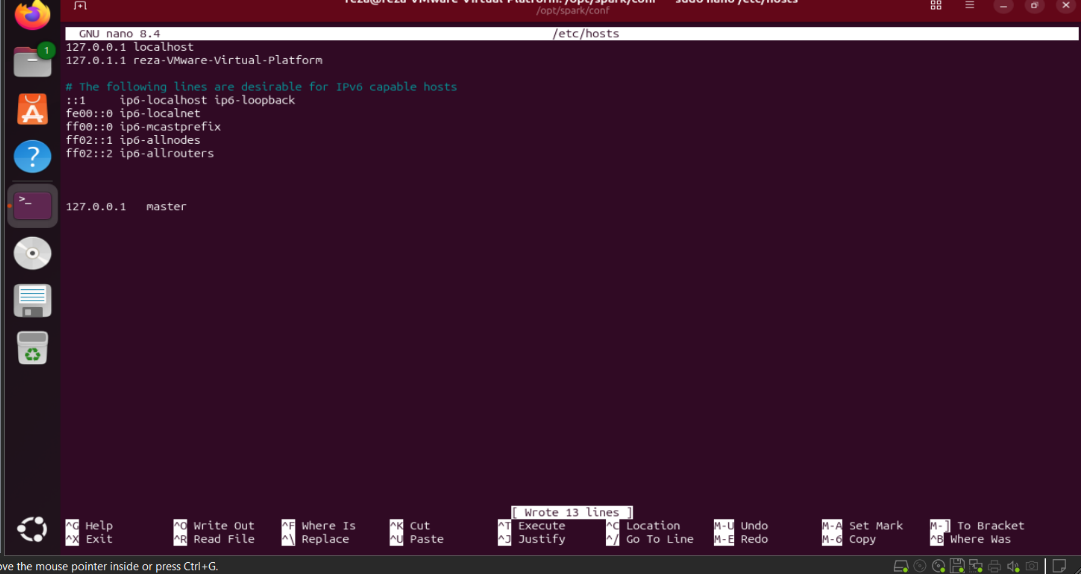
\includegraphics[width=\linewidth,height=.72\textheight,keepaspectratio]{assets/041_p031_02.png}\caption{Implementation and output: Master/worker configuration and final integration.}\label{fig:041_p031_020}\end{figure}
\begin{figure}[!htbp]\centering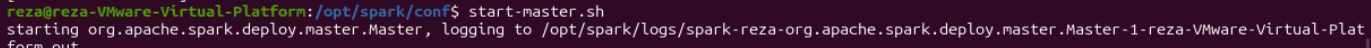
\includegraphics[width=\linewidth,height=.72\textheight,keepaspectratio]{assets/041_p032_01.png}\caption{Implementation and output: Master/worker configuration and final integration.}\label{fig:041_p032_010}\end{figure}
\begin{figure}[!htbp]\centering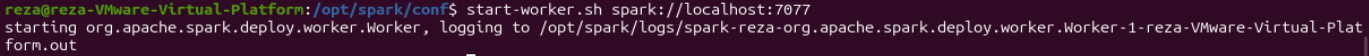
\includegraphics[width=\linewidth,height=.72\textheight,keepaspectratio]{assets/041_p032_02.png}\caption{Implementation and output: Master/worker configuration and final integration.}\label{fig:041_p032_020}\end{figure}
\begin{figure}[!htbp]\centering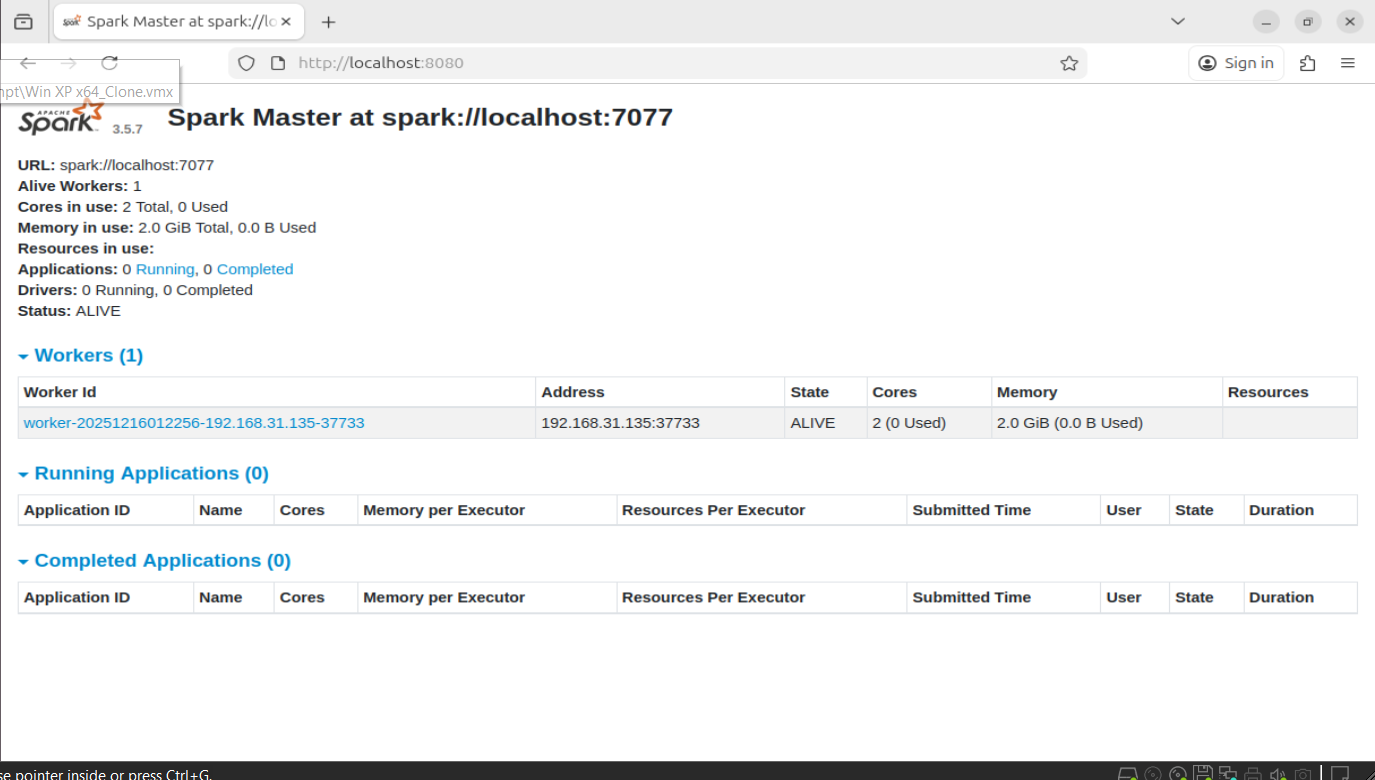
\includegraphics[width=\linewidth,height=.72\textheight,keepaspectratio]{assets/041_p032_03.png}\caption{Implementation and output: Master/worker configuration and final integration.}\label{fig:041_p032_030}\end{figure}
\begin{figure}[!htbp]\centering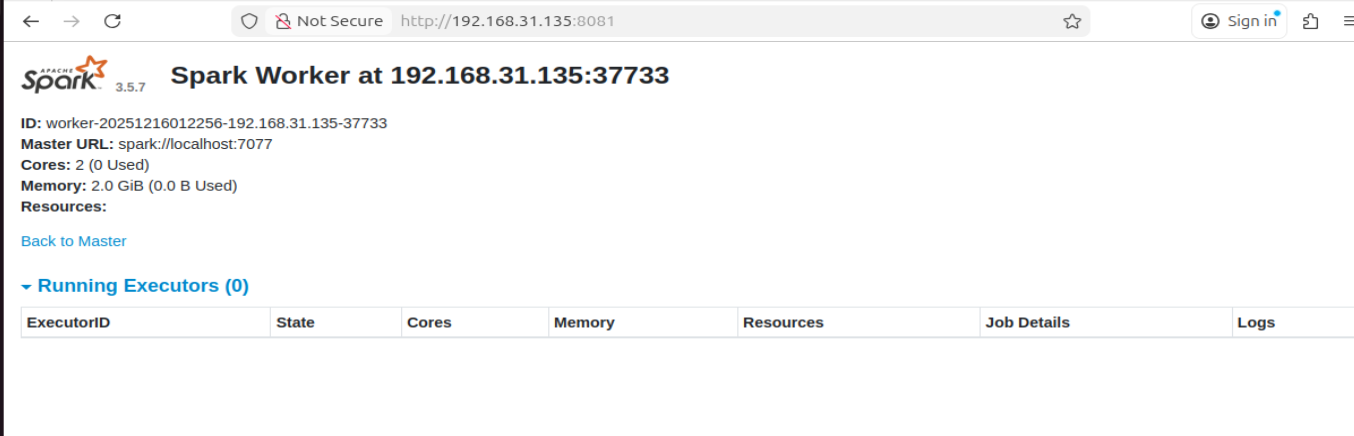
\includegraphics[width=\linewidth,height=.72\textheight,keepaspectratio]{assets/041_p033_01.png}\caption{Implementation and output: Master/worker configuration and final integration.}\label{fig:041_p033_010}\end{figure}
\begin{figure}[!htbp]\centering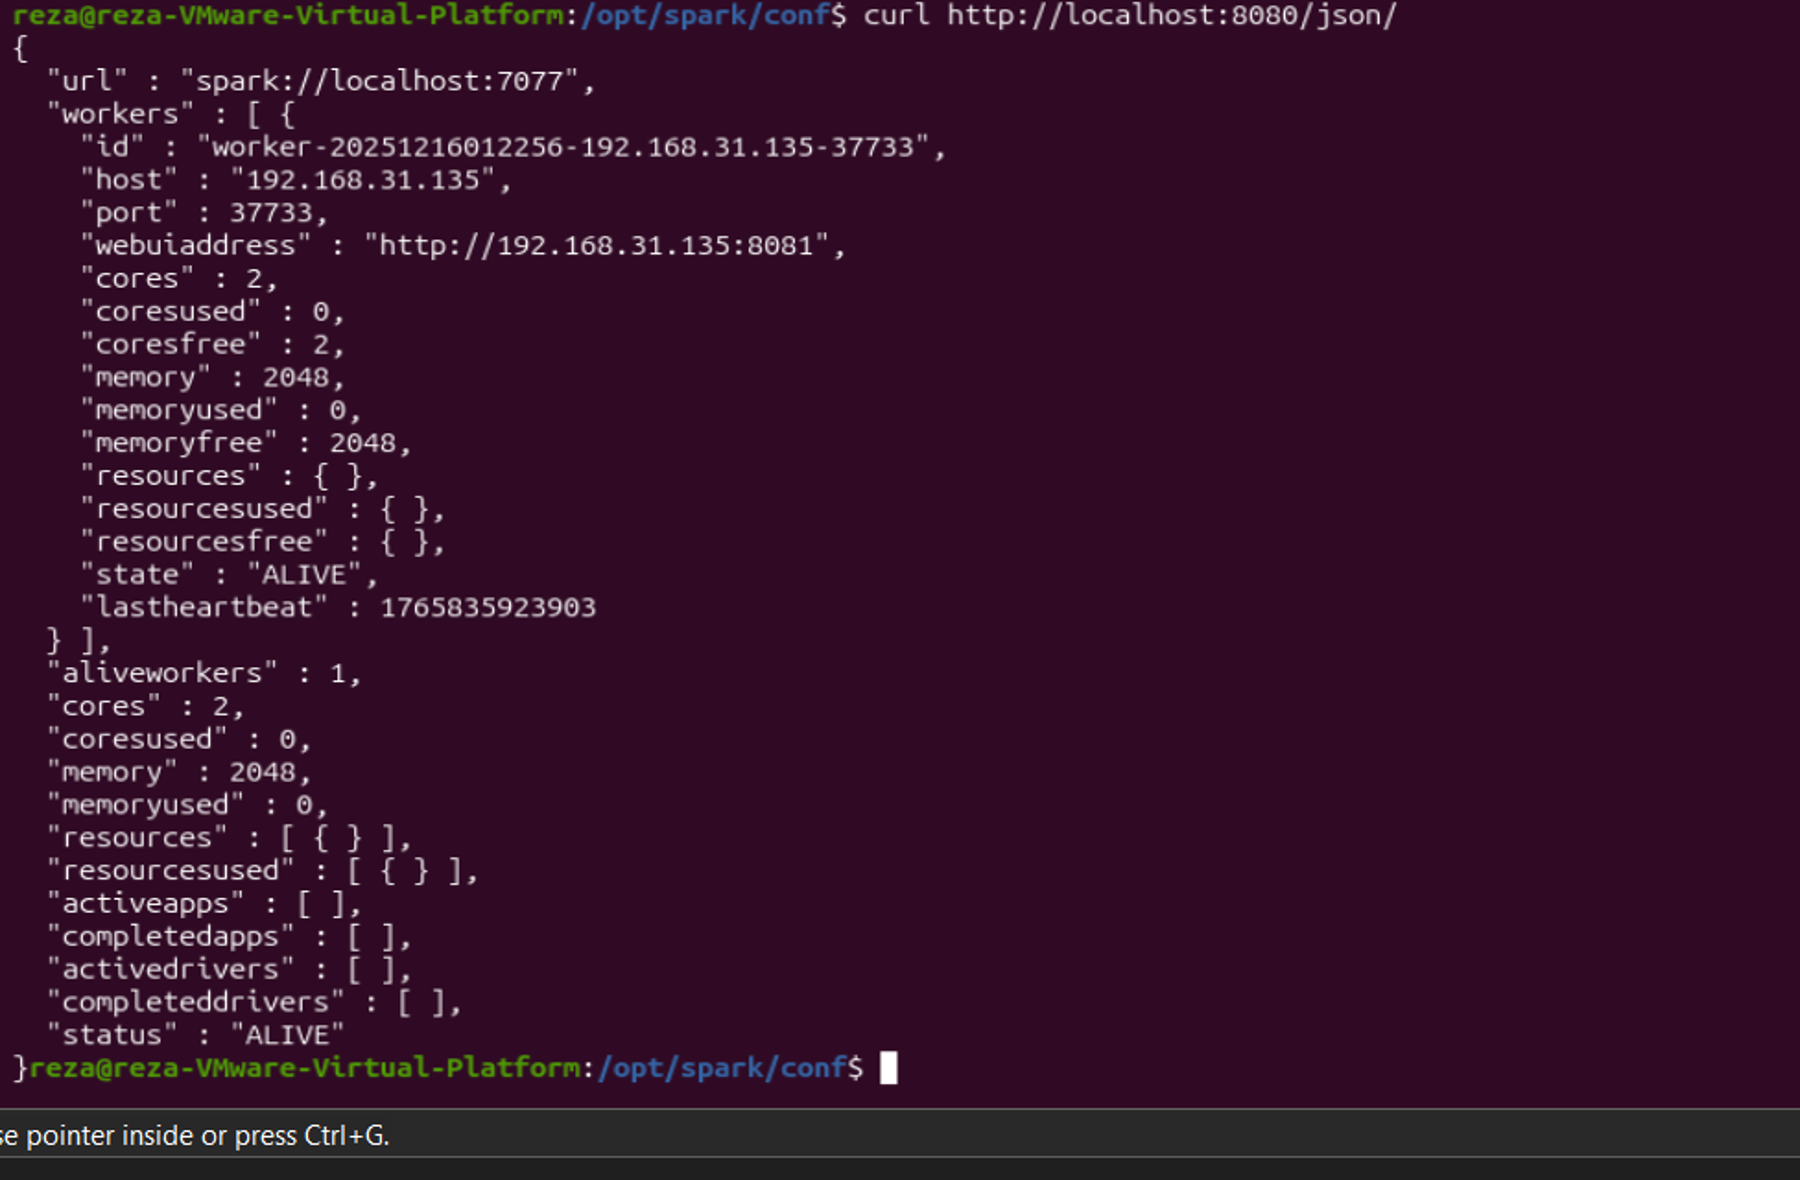
\includegraphics[width=\linewidth,height=.72\textheight,keepaspectratio]{assets/041_p033_02.png}\caption{Implementation and output: Master/worker configuration and final integration.}\label{fig:041_p033_020}\end{figure}
\begin{figure}[!htbp]\centering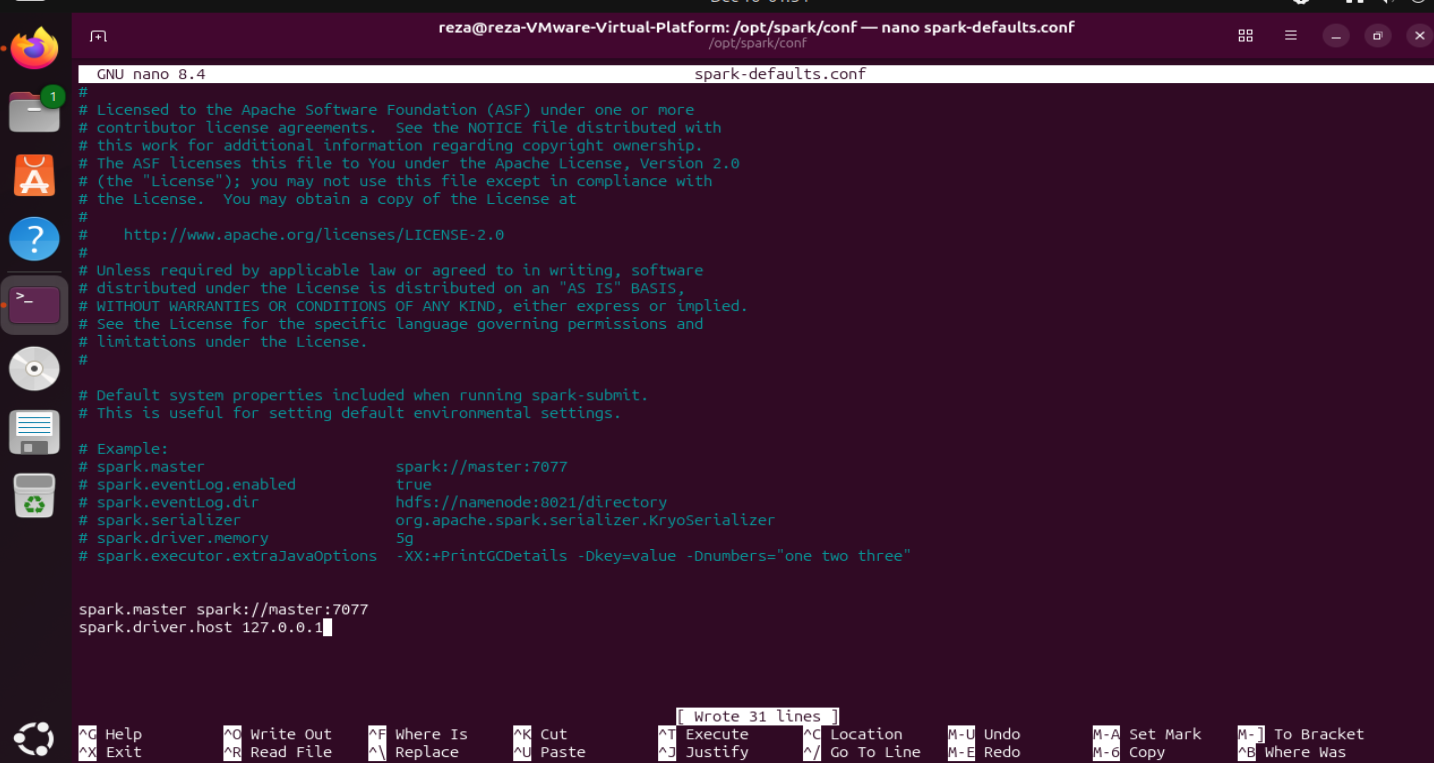
\includegraphics[width=\linewidth,height=.72\textheight,keepaspectratio]{assets/041_p034_01.png}\caption{Implementation and output: Master/worker configuration and final integration.}\label{fig:041_p034_010}\end{figure}
\begin{figure}[!htbp]\centering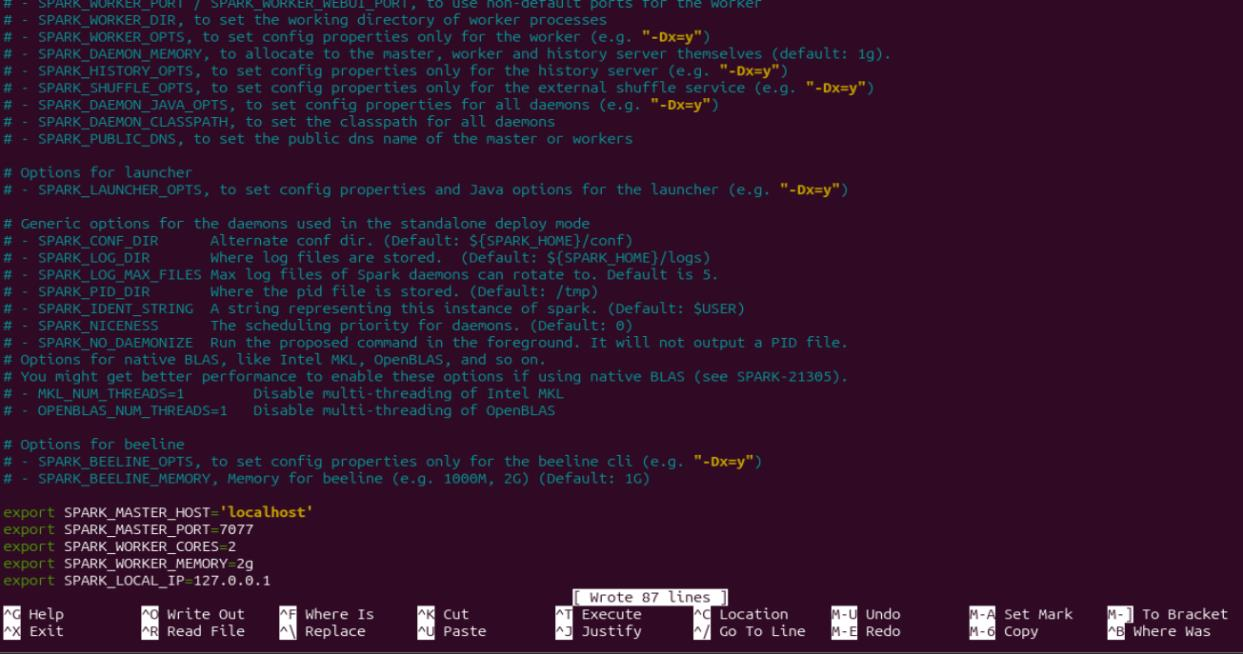
\includegraphics[width=\linewidth,height=.72\textheight,keepaspectratio]{assets/041_p035_01.png}\caption{Implementation and output: Master/worker configuration and final integration.}\label{fig:041_p035_010}\end{figure}
\begin{figure}[!htbp]\centering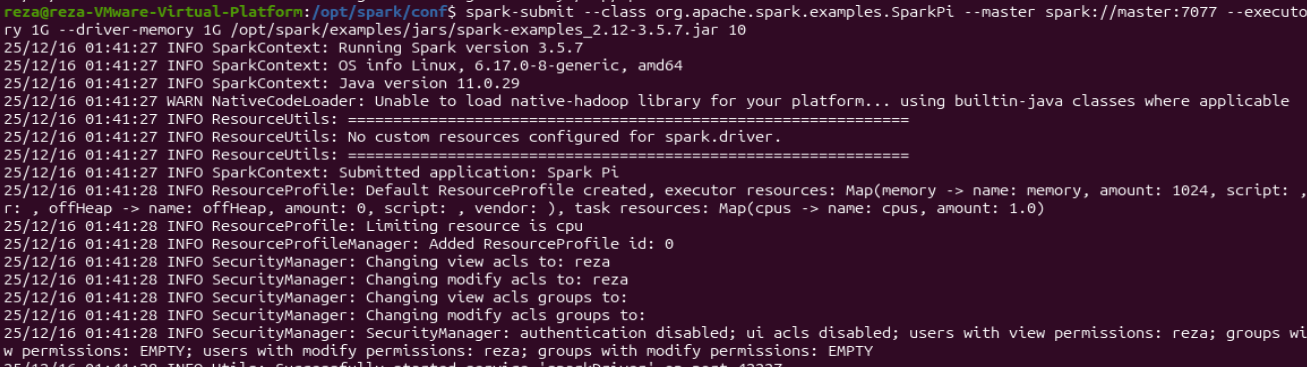
\includegraphics[width=\linewidth,height=.72\textheight,keepaspectratio]{assets/041_p035_02.png}\caption{Implementation and output: Master/worker configuration and final integration.}\label{fig:041_p035_020}\end{figure}
\begin{figure}[!htbp]\centering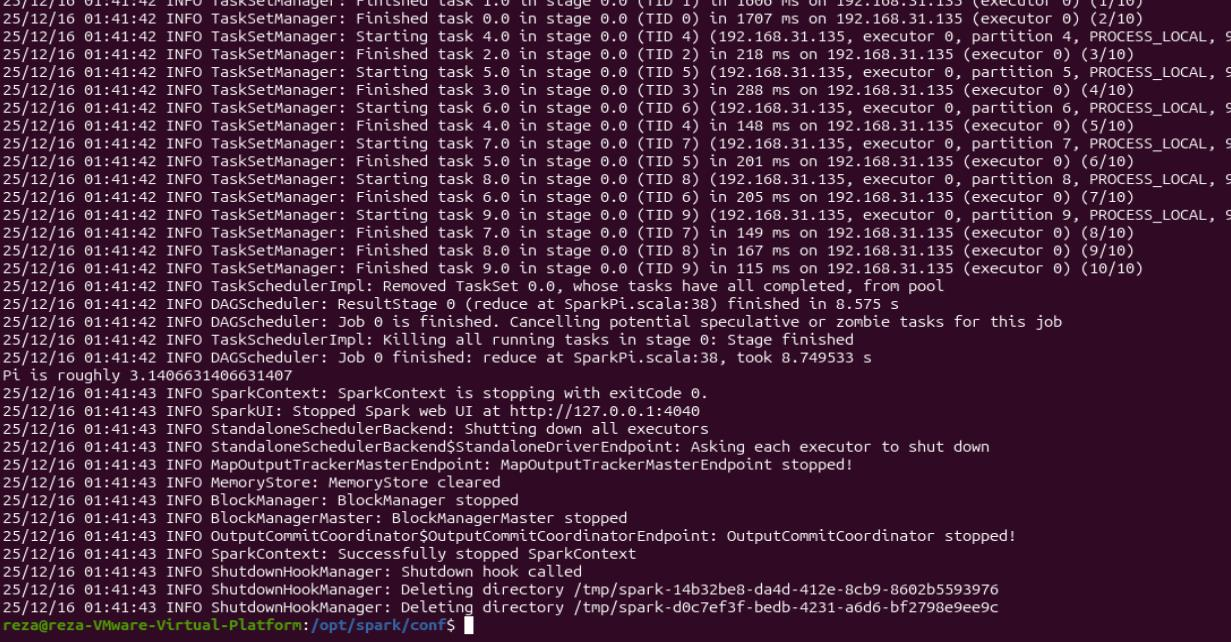
\includegraphics[width=\linewidth,height=.72\textheight,keepaspectratio]{assets/041_p036_01.png}\caption{Implementation and output: Master/worker configuration and final integration.}\label{fig:041_p036_010}\end{figure}
\clearpage
\end{document}